% This is a clean template for a Springer LNCS paper
\documentclass[runningheads]{llncs}

\usepackage[T1]{fontenc}
\usepackage{graphicx}
\usepackage{amsmath,amssymb}
\usepackage{booktabs}
\usepackage{array}
% If you use the hyperref package, please uncomment the following two lines
% to display URLs in blue roman font according to Springer's eBook style:
%\usepackage{color}
%\renewcommand\UrlFont{\color{blue}\rmfamily}
%\urlstyle{rm}

\begin{document}

\title{Detecting Equatorial Plasma Bubbles with Machine Learning}

% \titlerunning{Abbreviated paper title}
% If the paper title is too long for the running head, you can set
% an abbreviated paper title here

\author{Alberto I C Vieira\inst{1}\orcidID{0009-0002-3711-9403} \and
Cosme A O B Figueiredo\inst{2}\orcidID{0000-0003-4423-5111} \and
Tiago M U Araújo\inst{1}\orcidID{0000-0002-5953-5435}}

\authorrunning{A. I. C. Vieira et al.}

\institute{Universidade Federal da Paraíba \and Universidade Federal de Campina Grande}

\maketitle              % typeset the header of the contribution

\begin{abstract}
Equatorial Plasma Bubbles (EPBs) produce ionospheric irregularities that cause radio scintillation and degrade GNSS and satellite communication links at low latitudes. Optical monitoring of EPBs still depends largely on visual inspection of $630.0\text{ nm}$ all-sky airglow images, a slow task made harder by moonlight, horizon brightening, and clouds. We describe a two-stage pipeline for automatic EPB detection. The first stage checks sky transparency by counting star pixels and measuring the mean sky brightness inside the field of view, and discards cloud-covered frames. The second stage removes the diffuse background, enhances local contrast with CLAHE, extracts features with Two-Dimensional Principal Component Analysis (2DPCA), and classifies them with a stacking ensemble of SVM, XGBoost, and Random Forest. On $572$ labeled images from three EMBRACE observatories in Brazil, the classifier reached $97.20\%$ accuracy and $0.998$ ROC-AUC under stratified 5-fold cross-validation, and $95.08\%$ accuracy when whole $30$-minute windows were held out. Without background normalization, recall on an observatory left out of training fell from $100\%$ to $0\%$, which indicates that the model then learns station brightness rather than plasma structure. On an overcast night excluded from training, the first stage flagged $79\%$ of the frames as cloudy and cut false alarms by $78.7$--$90.2\%$. SHAP maps projected back to pixel space show that the predictions follow the north--south depletion bands.

\keywords{Equatorial Plasma Bubbles \and Machine Learning \and Space Weather \and All-Sky Imager \and 2DPCA \and Stacking Ensemble \and Explainable AI.}
\end{abstract}

\section{Introduction}\label{sec:introduction}

Equatorial Plasma Bubbles (EPBs) are large regions of depleted plasma density that form in the equatorial F region after sunset through the generalized Rayleigh-Taylor instability. Once the Sun sets, recombination quickly erodes the bottomside ionosphere and leaves a steep upward density gradient beneath the F layer. When the pre-reversal enhancement of the eastward electric field is strong, this configuration becomes unstable: low-density plasma rises into the topside ionosphere as plumes that extend to low latitudes and drift eastward. The small-scale irregularities inside these depletions cause amplitude and phase scintillation in radio signals, degrading GNSS positioning and satellite communications \cite{zhong2025automatic,okoh2025bootstrapping,githio2024machine}.

From the ground, EPBs are usually observed with All-Sky Imagers (ASIs) fitted with narrow-band filters at $630.0\text{ nm}$, the atomic oxygen red line emitted at about $250\text{--}300\text{ km}$ \cite{okoh2025bootstrapping,zhong2025automatic}. Because the emission is weaker inside the depletions, bubbles appear as dark bands elongated in the north--south direction. At an observatory, finding them still means looking through hundreds of images per night. The task is slow, and it becomes ambiguous when faint depletions overlap with moonlight, horizon brightening from the Van Rhijn effect, the Milky Way, or passing clouds.

Several recent works have applied machine learning to this problem. Convolutional Neural Networks (CNNs) and segmentation models have been used to classify EPB occurrence, track medium-scale traveling ionospheric disturbances, and build multi-year climatologies \cite{srisamoodkham2022detecting,liu2022statistical,sedlak2023analysis,okoh2025bootstrapping,zhong2025automatic,zhong2025statistical}, and other studies combined CNN feature extractors with Support Vector Machines (SVMs) or with collocated GNSS scintillation data \cite{thanakulketsarat2023classification,thanakulketsarat2023equatorial,githio2024machine}. Deep networks, however, are costly to train and, on the moderate, station-specific datasets typical of optical observatories, are prone to shortcut learning: they may pick up background brightness, dome structures, or the timestamp printed on the image instead of the shape of the depletion. A lighter alternative is Two-Dimensional Principal Component Analysis (2DPCA) \cite{yang2004two}, which works directly on the image matrix and keeps part of its spatial structure. Yacoub et al. \cite{yacoub2025automatic} and Siddiqui \cite{siddiqui2025enhanced} recently combined 2DPCA with tree-based and ensemble classifiers for airglow images.

Three practical problems remain. First, local contrast enhancement turns dark cloud edges into sharp bands that classifiers confuse with EPBs, so cloudy frames have to be removed before classification. Second, consecutive exposures, taken $3\text{--}5$ minutes apart, are strongly correlated; random frame-level splits can therefore overestimate performance unless the model is also tested on held-out time windows and on stations not seen during training. Third, all-sky images carry the station code and timestamp burned into their corners, and one must check that the classifier does not rely on them.

This paper proposes a two-stage pipeline for EPB detection in $630.0\text{ nm}$ images from the Brazilian EMBRACE network. The first stage is a sky quality check, based on star counts and sky brightness, that discards cloud-covered frames. The second stage normalizes the background and local contrast, projects the image onto a small 2DPCA subspace, and classifies it with a stacking ensemble \cite{wolpert1992stacked}. We evaluate the pipeline with stratified, time-grouped, and text-masked cross-validation, with zero-shot transfer to an unseen station, and on full-night sequences, and we inspect its decisions with 2DPCA reconstruction residuals and SHapley Additive exPlanations (SHAP) \cite{lundberg2017unified}. Section~\ref{sec:methodology} describes the data and the method, Section~\ref{sec:results} presents the results, and Section~\ref{sec:conclusion} concludes the paper.

\section{Methodology}\label{sec:methodology}

The system works as a two-stage cascade (Figure~\ref{fig:pipeline_arch}). Stage~1 measures sky transparency on the raw exposure and holds back cloud-covered frames. The frames that pass go to Stage~2, where radiometric preprocessing, 2DPCA projection, and a stacking ensemble estimate the probability that an EPB is present.

\begin{figure}[htbp]
    \centering
    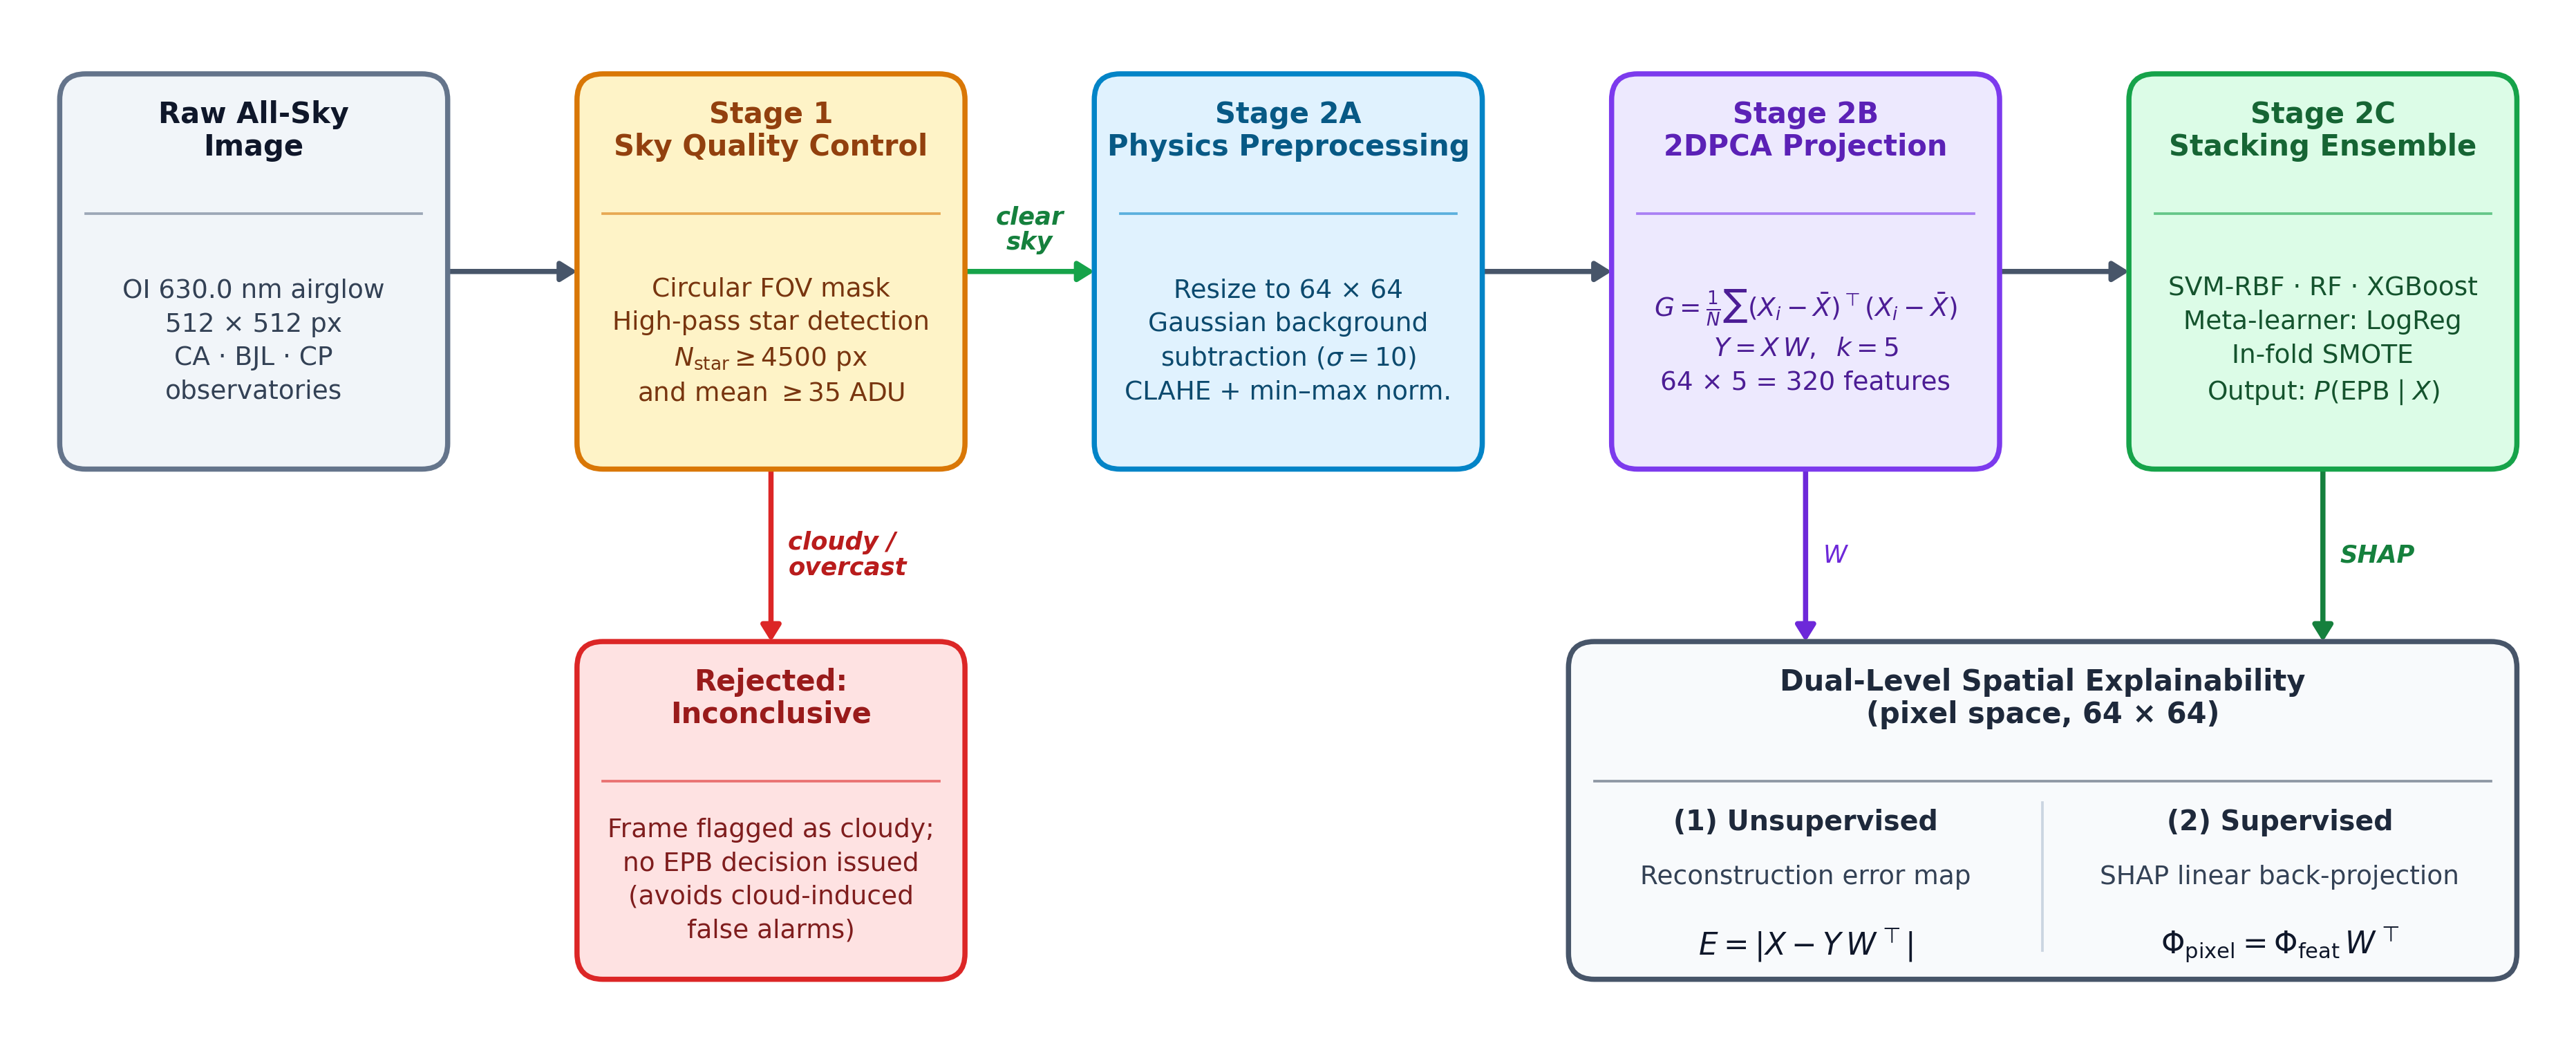
\includegraphics[width=0.98\textwidth]{figs/pipeline_architecture.png}
    \caption{Overview of the two-stage cascaded EPB detection pipeline. Stage~1 screens out cloud-contaminated exposures using star-pixel counts and mean luminance inside the circular field of view; Stage~2 applies background subtraction and CLAHE, extracts 2DPCA matrix features ($k=5$, $320$ features), and classifies frames with a stacking ensemble.}
    \label{fig:pipeline_arch}
\end{figure}

\subsection{Dataset}\label{sec:data}

The images come from the \textit{Estudo e Monitoramento Brasileiro do Clima Espacial} (EMBRACE) program of the Brazilian National Institute for Space Research (INPE). The instruments are all-sky CCD imagers with fish-eye lenses ($180^\circ$ field of view) and a narrow-band $630.0\text{ nm}$ filter. Each exposure is an $8$-bit $512 \times 512$ grayscale image, recorded every $3\text{--}5$ minutes.

\begin{table}[htbp]
\centering
\caption{Summary of the EMBRACE $630.0\text{ nm}$ all-sky dataset across observatories, lunar illumination regimes, and continuous nocturnal monitoring sequences.}
\label{tab:dataset}
\resizebox{\textwidth}{!}{%
\setlength{\tabcolsep}{5pt}
\begin{tabular}{llrrrr}
\toprule
\textbf{Dataset Subset / Observatory} & \textbf{Coordinates} & \textbf{Total} & \textbf{EPB} & \textbf{No-EPB} & \textbf{EPB (\%)} \\
\midrule
\multicolumn{6}{l}{\textit{Part A: Labeled Classification Dataset ($N = 572$ images, $16$ nights, $77$ temporal blocks)}} \\
São João do Cariri (CA) & $7.4^\circ\text{S}, 36.5^\circ\text{W}$ & 310 & 213 & 97 & 68.7\% \\
Bom Jesus da Lapa (BJL) & $13.3^\circ\text{S}, 43.4^\circ\text{W}$ & 220 & 0 & 220 & 0.0\% \\
Cachoeira Paulista (CP) & $22.7^\circ\text{S}, 45.0^\circ\text{W}$ & 42 & 42 & 0 & 100.0\% \\
\quad Low/Moderate Moon ($<50\%$) & All stations & 475 & 255 & 220 & 53.7\% \\
\quad Bright Lunar Glare ($\ge 50\%$) & All stations & 97 & 0 & 97 & 0.0\% \\
\textbf{Total Labeled Dataset} & \textbf{3 Stations} & \textbf{572} & \textbf{255} & \textbf{317} & \textbf{44.6\%} \\
\midrule
\multicolumn{6}{l}{\textit{Part B: Continuous Nocturnal Sequences ($986$ total frames across $8$ nights)}} \\
\texttt{BJL\_20250722} (Clear Quiet Sky) & $13.3^\circ\text{S}, 43.4^\circ\text{W}$ & 230 & 0 & 230 & 0.0\% \\
\texttt{CA\_20251022} (Active EPB Night) & $7.4^\circ\text{S}, 36.5^\circ\text{W}$ & 140 & 126 & 14 & 90.0\% \\
\texttt{CA\_20260624} (Overcast / Cloudy) & $7.4^\circ\text{S}, 36.5^\circ\text{W}$ & 62 & 0 & 62 & 0.0\% \\
Five Additional Monitoring Nights & CA / BJL / CP & 554 & -- & -- & Operational \\
\bottomrule
\end{tabular}%
}
\end{table}

The data are divided into two parts (Table~\ref{tab:dataset}). Part~A contains $572$ images labeled by an expert ($255$ with EPBs and $317$ without, a negative-to-positive ratio of $1.24:1$), taken on $16$ nights and grouped into $77$ non-overlapping $30$-minute windows. They come from three observatories at different magnetic latitudes: São João do Cariri (CA), Bom Jesus da Lapa (BJL), and Cachoeira Paulista (CP). The class balance differs a lot between sites, since BJL contributes only negative examples and CP only positive ones. A model that works on raw intensities could therefore separate the classes just by recognizing the station from its background brightness. Of the negatives from CA, $62$ were recorded under overcast skies. In addition, $97$ negatives ($17.0\%$ of Part~A) were taken with the Moon at least $50\%$ illuminated (fraction computed from each timestamp), when glare produces strong brightness gradients across the dome. Part~B has eight full-night sequences ($986$ frames), used to test temporal stability and cloud rejection.

\subsection{Stage 1: Sky Quality Control}\label{sec:stage1}

Clouds attenuate the $630.0\text{ nm}$ emission and create dark patches that, after contrast enhancement, look like plasma depletions. Stars give a simple measure of transparency: on a clear night many point sources are visible across the dome, while clouds blur or hide them.

Each raw $512 \times 512$ image $I_{\text{raw}}$, with values in $[0, 255]$, is restricted to a circular mask of radius $r = 0.44 \min(H, W)$ centered on the dome, which leaves out the station code and timestamp printed in the corners. To separate stars from the diffuse sky, we smooth the image with a Gaussian filter ($\sigma = 2.0$ pixels) and take the high-pass residual
\begin{equation}\label{eq:star_residual}
    R_{\text{high}}(x, y) = I_{\text{raw}}(x, y) - (G_{\sigma=2.0} * I_{\text{raw}})(x, y).
\end{equation}
A pixel $(x, y)$ inside the mask is counted as a star pixel if $R_{\text{high}}(x, y) > 8.0$ and $I_{\text{raw}}(x, y) > 30.0$, where the intensity threshold keeps dark-current noise in dark regions from being counted as stars. Let $N_{\text{star}}$ be the number of star pixels and $\mu_{\text{sky}}$ the mean of $I_{\text{raw}}$ inside the mask. A frame is labeled \texttt{CLOUDY} and discarded if $\mu_{\text{sky}} < 35.0$ or $N_{\text{star}} < 4500$. Frames with $4500 \le N_{\text{star}} < 6500$ go to Stage~2 with a partial-visibility flag (\texttt{DEGRADED}), and frames with $N_{\text{star}} \ge 6500$ go as \texttt{CLEAR}.

\subsection{Stage 2: Preprocessing, Augmentation, and Balancing}\label{sec:stage2}

Frames accepted by Stage~1 are resized to $64 \times 64$ pixels (bilinear interpolation), scaled to $[0, 1]$, and go through three steps meant to remove brightness variations that do not come from the ionosphere:
\begin{enumerate}
    \item Background subtraction: all-sky images show radial brightening toward the horizon (Van Rhijn effect) and smooth gradients from moonlight. We estimate this slowly varying component with a Gaussian filter ($\sigma = 10$ pixels) and subtract it, clipping negative values at zero: $I_{\text{sub}}(x,y) = \max\!\big(0,\, I(x,y) - (G_{\sigma=10} * I)(x,y)\big)$.
    \item Contrast equalization: Contrast Limited Adaptive Histogram Equalization (CLAHE, clip limit $0.03$) is applied to $I_{\text{sub}}$, so that faint depletion bands stand out without amplifying noise in uniform regions of the sky.
    \item Normalization and optional masking: the result is min-max normalized to $[0, 1]$, giving the input matrix $\mathbf{X} \in \mathbb{R}^{64 \times 64}$. To test the influence of the corner text, we also build a masked version $\mathbf{X}_{\text{mask}}$ in which all pixels outside $r = 0.44 \times 64$ are set to zero.
\end{enumerate}

The data are split before any augmentation, subspace fitting, or oversampling. Only training images are augmented, with transformations compatible with all-sky geometry: small rotations ($\pm 15^\circ$), horizontal flips, slight changes in brightness and contrast ($\pm 10\%$), and weak Gaussian noise ($\sigma = 0.02$). After 2DPCA extraction and z-score standardization (fitted on the training fold only), the Synthetic Minority Over-sampling Technique (SMOTE) \cite{chawla2002smote} balances the classes inside an \texttt{imblearn} pipeline, again on the training fold only. Validation and test sets are never augmented or resampled.

\subsection{2DPCA Projection, Stacking Ensemble, and Explainability}\label{sec:model}

Flattening a $64 \times 64$ image into a $4096$-dimensional vector loses the spatial neighborhood and requires estimating a $4096 \times 4096$ covariance matrix from a few hundred samples. 2DPCA \cite{yang2004two} instead computes a $64 \times 64$ image covariance matrix directly from the centered training matrices $\{\mathbf{X}_i \in \mathbb{R}^{64 \times 64}\}_{i=1}^{M}$ with sample mean $\bar{\mathbf{X}} = \frac{1}{M}\sum_{i=1}^{M} \mathbf{X}_i$:
\begin{equation}\label{eq:2dpca_cov}
    \mathbf{G} = \frac{1}{M}\sum_{i=1}^{M} (\mathbf{X}_i - \bar{\mathbf{X}})^\top (\mathbf{X}_i - \bar{\mathbf{X}}) \in \mathbb{R}^{64 \times 64}.
\end{equation}
Let $\mathbf{W} = [\mathbf{w}_1, \mathbf{w}_2, \dots, \mathbf{w}_k] \in \mathbb{R}^{64 \times k}$ contain the orthonormal eigenvectors of $\mathbf{G}$ associated with the $k$ largest eigenvalues $\lambda_1 \ge \lambda_2 \ge \dots \ge \lambda_k$. Projecting a centered image onto $\mathbf{W}$ yields the principal component matrix $\mathbf{Y}_i = (\mathbf{X}_i - \bar{\mathbf{X}})\mathbf{W} \in \mathbb{R}^{64 \times k}$. Each entry $Y_i(r, c)$, denoted as feature \texttt{PC\_Row\_$r$\_Comp\_$c$}, is the projection of image row $r \in \{0, \dots, 63\}$ onto the eigenvector $\mathbf{w}_c$ ($c \in \{0, \dots, k-1\}$); the row order is kept and only the horizontal variation is compressed. With $k=5$, chosen by cross-validation (Section~\ref{sec:kselect}), vectorizing $\mathbf{Y}_i$ gives a $320$-dimensional feature vector $\mathbf{z}_i$, $12.8$ times smaller than the image.

The standardized vector $\mathbf{z}_i$ is classified by a two-level stacking ensemble \cite{wolpert1992stacked} with three base learners:
\begin{enumerate}
    \item A Support Vector Machine (SVM) with a Radial Basis Function (RBF) kernel ($C = 5.0$, $\gamma = \text{scale}$, balanced class weights).
    \item An XGBoost classifier ($200$ trees, maximum depth $6$, learning rate $0.1$, subsample $0.8$, column subsample $0.8$).
    \item A Random Forest classifier ($200$ trees, maximum depth $15$, minimum leaf size $2$, balanced class weights).
\end{enumerate}
The out-of-fold probabilities of the three learners, obtained by an internal 5-fold cross-validation, are combined by an $\ell_2$-regularized Logistic Regression ($C = 1.0$).

To see where in the image the decisions come from, we use two maps. The first is unsupervised: reconstructing the image from its projection, $\hat{\mathbf{X}}_i = \bar{\mathbf{X}} + \mathbf{Y}_i \mathbf{W}^\top$, gives the error map $\mathbf{E}_i = |\mathbf{X}_i - \hat{\mathbf{X}}_i|$, which highlights local structures that the leading components do not capture. The second is supervised: we compute SHAP values \cite{lundberg2017unified} for the tree learners in the $320$-dimensional feature space, reshape them into $\boldsymbol{\Phi}_{\text{feat}} \in \mathbb{R}^{64 \times k}$, and, since 2DPCA is linear, map them back to pixels with $\boldsymbol{\Phi}_{\text{pixel}} = \boldsymbol{\Phi}_{\text{feat}}\mathbf{W}^\top$. Positive values mark pixels that raise the EPB probability, and negative values mark pixels that favor a quiet sky.

\subsection{Evaluation Protocol}\label{sec:protocol}

We report 5-fold stratified cross-validation on the $572$ labeled images and the results on a stratified holdout split with $25\%$ of the data ($n=143$). Because consecutive frames are correlated, we also run a 5-fold group cross-validation in which all frames of a $30$-minute window fall in the same fold (temporal-block CV), and we repeat the stratified CV on the masked inputs $\mathbf{X}_{\text{mask}}$ to check the effect of the corner text. Transfer between sites is measured by training on CA and BJL ($n=530$) and testing on CP ($n=42$) without any retraining (zero-shot). As CP has only EPB frames, this test measures recall only.

The pipeline is compared with classifiers on flattened pixels ($4096$ features) and on 1D-PCA ($320$ components), with each 2DPCA base learner used alone, and with a small 2D CNN ($\text{AvgPool}_{2\times 2} \to \text{Conv2D}_{8,5\times 5} \to \text{MaxPool}_{2\times 2} \to \text{Conv2D}_{16,3\times 3} \to \text{MaxPool}_{2\times 2} \to \text{Dense}_{32} \to \text{Sigmoid}$, trained for $25$ epochs with Adam). We also run three ablations: without radiometric preprocessing, without SMOTE, and with the circular mask. For the full-night tests with clouds, Stage~2 is retrained on the $510$ labeled images without cloud cover, so that no overcast frame is seen during training. We report accuracy, sensitivity (recall), specificity, precision, F1-score, ROC-AUC, PR-AUC, and CPU inference time per image.

\section{Results}\label{sec:results}

We first discuss the choice of $k$ and the 2DPCA reconstructions, then the cross-validation results, the comparison with baselines and ablations, the tests under moonlight and clouds, and finally the SHAP maps and full-night time series.

\subsection{2DPCA Spectrum and Reconstruction Residuals}\label{sec:kselect}

To choose the number of projection vectors $k$, we looked at the eigenvalue spectrum of the image covariance matrix together with the 5-fold cross-validated F1-score on the training split for $k \in \{1, 2, 3, 5, 10, 15, 20, 25, 30\}$ (Figure~\ref{fig:2dpca_variance}).

\begin{figure}[htbp]
    \centering
    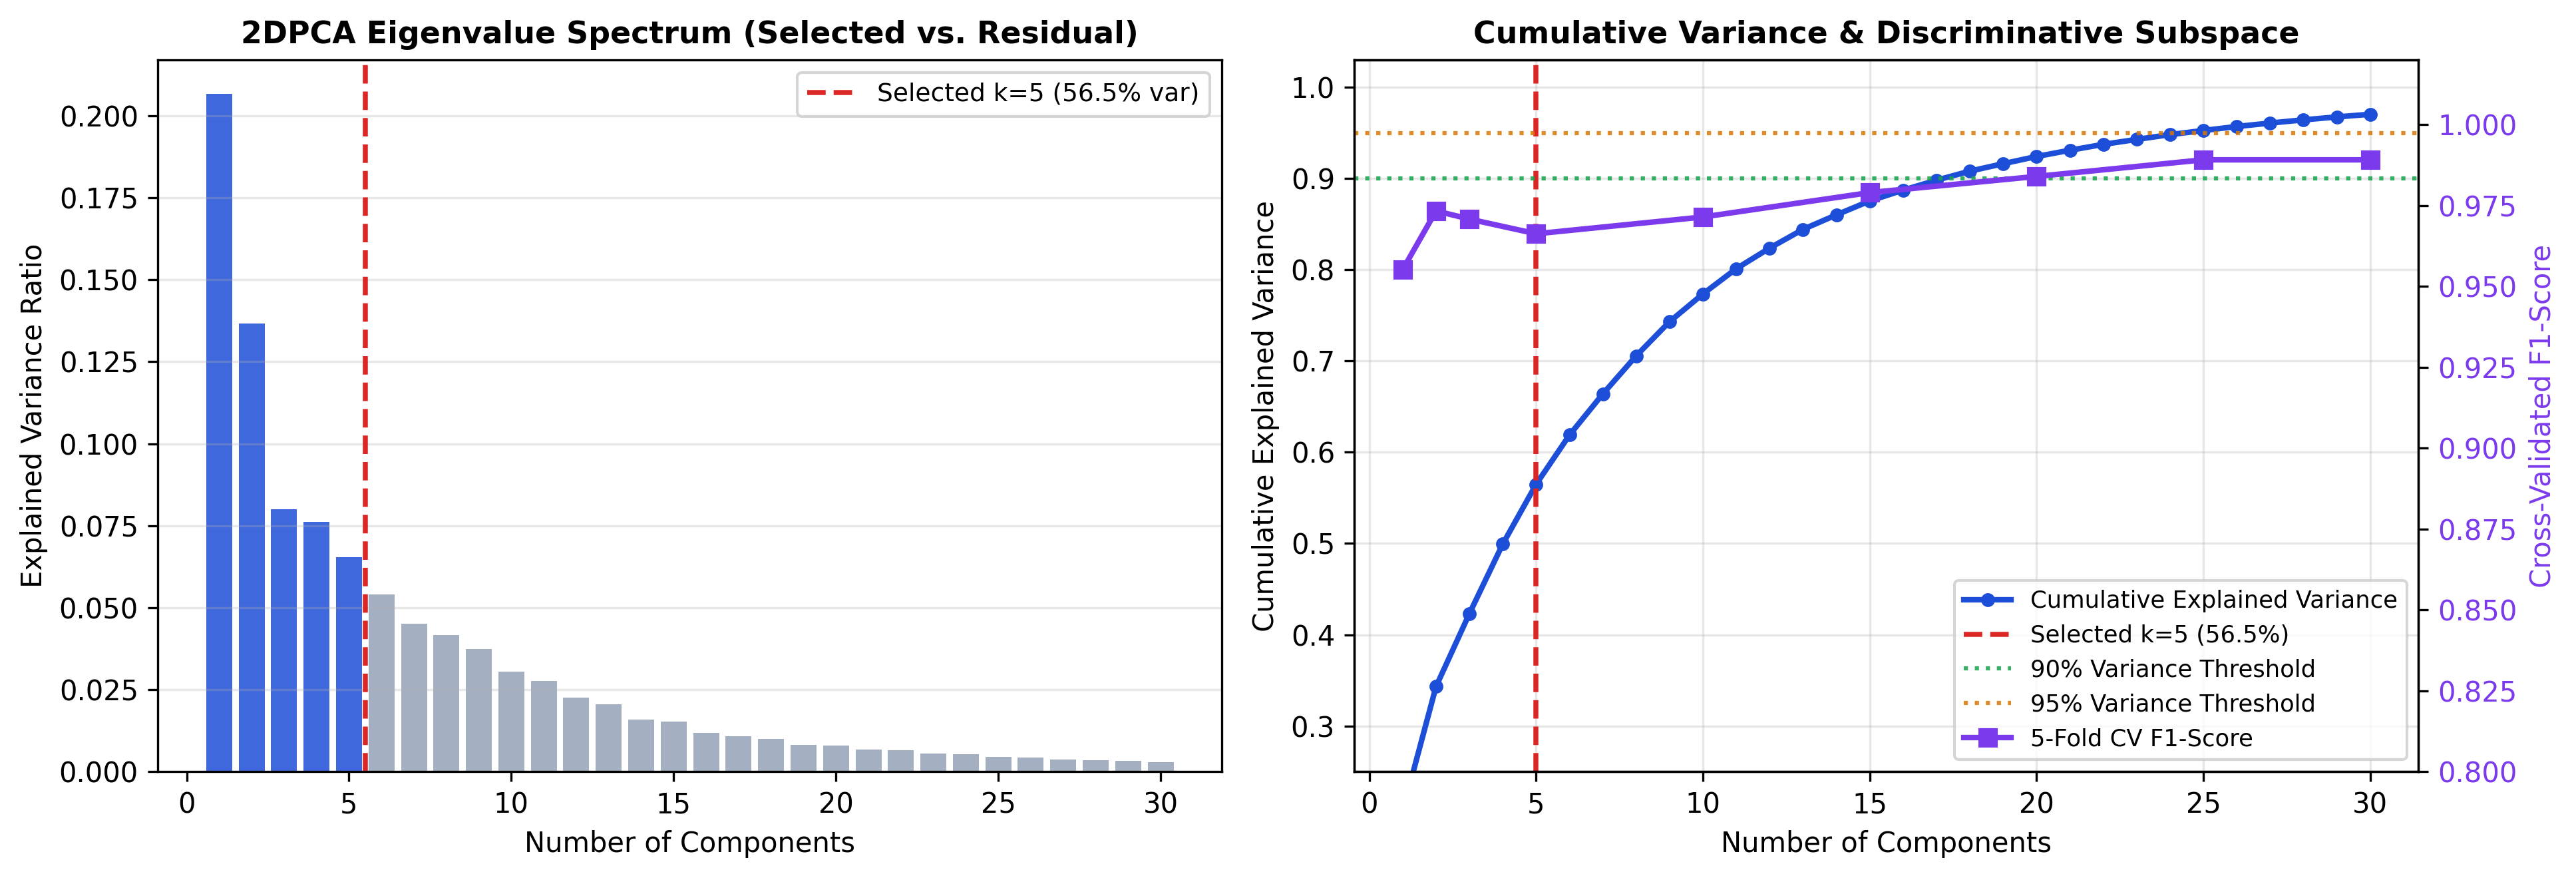
\includegraphics[width=0.98\textwidth]{figs/2dpca_variance.png}
    \caption{Left: Individual explained variance ratio across the first $30$ 2DPCA components (out of $64$) on the augmented training split, indicating the selected $k=5$ cutoff ($56.5\%$ cumulative variance). Right: Cumulative explained variance and 5-fold cross-validated F1-score from $k=1$ to $k=30$.}
    \label{fig:2dpca_variance}
\end{figure}

Since background subtraction and CLAHE are applied before the covariance is estimated, the uniform illumination mode, which accounts for nearly $80\%$ of the variance of raw images, is no longer present, and the variance spreads over more components. On the unaugmented training set ($n=429$), the cumulative variance goes from $22.86\%$ at $k=1$ to $59.41\%$ at $k=5$, $79.03\%$ at $k=10$, and $95.69\%$ at $k=25$. The components beyond $k=5$ mostly add fine-scale variance from residual stars and sensor grain, while the F1-score already exceeds $0.966$ at $k=5$. We therefore kept $k=5$ ($320$ features), which retains the mesoscale structure of the depletions and avoids the $1600\text{--}1920$ features required at $k=25\text{--}30$, a large number for a few hundred training images.

\begin{figure}[htbp]
    \centering
    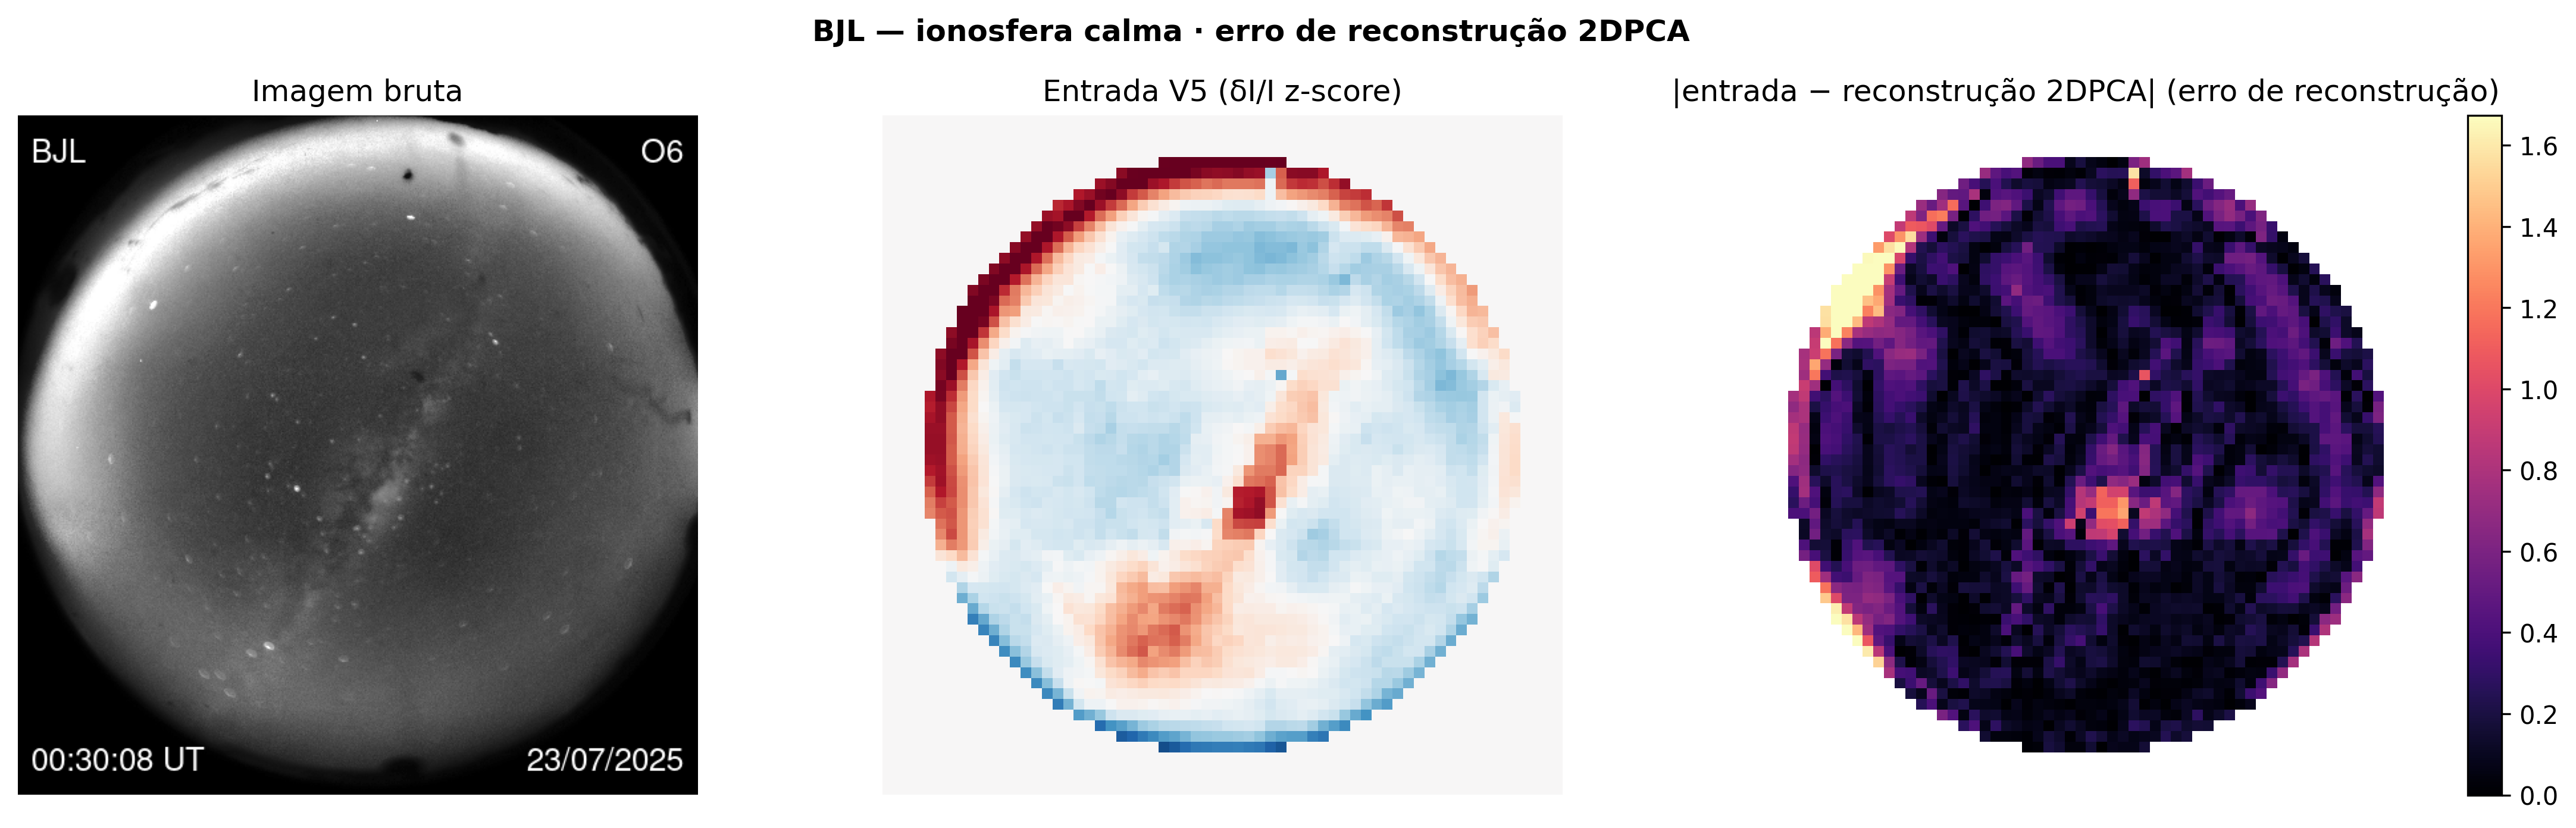
\includegraphics[width=0.96\textwidth]{figs/recon_error_without.png}
    \caption{Unsupervised 2DPCA subspace reconstruction analysis for a quiet-sky exposure (No EPB, predicted EPB probability $0.4\%$). Left: raw $630.0\text{ nm}$ image. Center: preprocessed $64 \times 64$ matrix $\mathbf{X}$. Right: reconstruction residual $|\mathbf{X} - \hat{\mathbf{X}}|$.}
    \label{fig:recon_error_without}
\end{figure}

\begin{figure}[htbp]
    \centering
    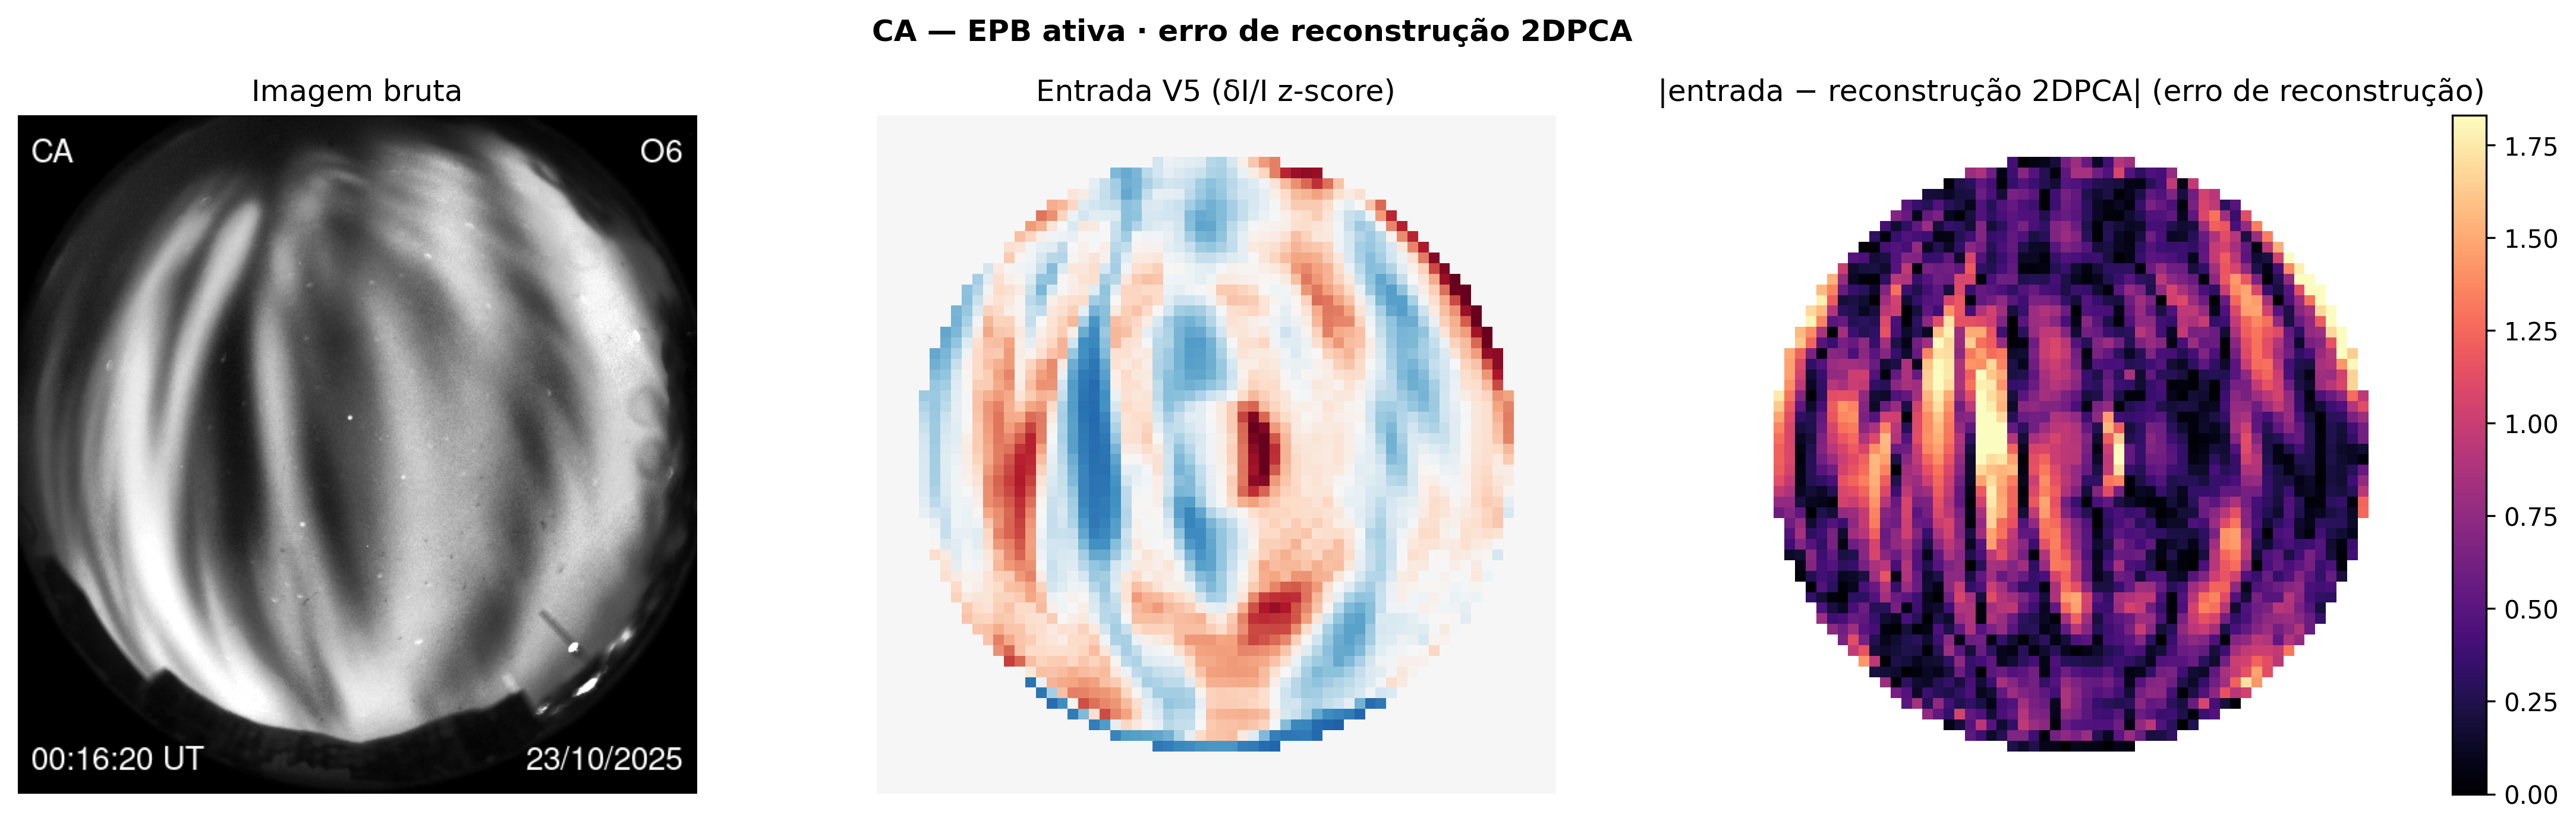
\includegraphics[width=0.96\textwidth]{figs/recon_error_with.png}
    \caption{Unsupervised 2DPCA subspace reconstruction analysis for an active EPB exposure (predicted EPB probability $99.2\%$). Large reconstruction residuals trace the North-South plasma depletion bands.}
    \label{fig:recon_error_with}
\end{figure}

Figures~\ref{fig:recon_error_without} and~\ref{fig:recon_error_with} show the $k=5$ reconstruction for a quiet and an active frame. In the quiet frame from BJL, the error is low inside the dome and appears only at the lens border and along a faint Milky Way streak. In the active frame from CA, the dark, bifurcated depletions create sharp intensity transitions, and the error exceeds $0.4$ along the whole north--south length of the bubbles.

\subsection{Cross-Validation Across Splitting Protocols}

Table~\ref{tab:cv_protocols} summarizes the results under each validation protocol. In stratified cross-validation (Figure~\ref{fig:kfold_cv}), the ensemble reached $97.20\%$ accuracy and $96.78\%$ F1-score, with specificity ($98.74\%$) higher than sensitivity ($95.30\%$); the PR-AUC was $0.9980 \pm 0.0018$. Pooling the out-of-fold predictions of all $572$ images (Figures~\ref{fig:confusion_matrix} and~\ref{fig:roc_pr}) gives only $4$ false positives against $12$ false negatives, so most errors are missed bubbles rather than false alarms. The holdout split ($64$ EPB and $79$ non-EPB images) gave similar numbers, with $96.50\%$ accuracy and a negative predictive value of $96.25\%$.

\begin{table}[htbp]
\centering
\caption{Performance of the 2DPCA ($k=5$) + Stacking Ensemble across validation protocols on the labeled dataset ($N=572$, mean $\pm$ standard deviation across folds).}
\label{tab:cv_protocols}
\resizebox{\textwidth}{!}{%
\setlength{\tabcolsep}{4pt}
\begin{tabular}{lcccccc}
\toprule
\textbf{Validation Protocol} & \textbf{Acc (\%)} & \textbf{Sens (\%)} & \textbf{Spec (\%)} & \textbf{Prec (\%)} & \textbf{F1 (\%)} & \textbf{ROC-AUC} \\
\midrule
5-Fold Stratified CV ($N=572$) & $97.20 \pm 1.57$ & $95.30 \pm 4.51$ & $98.74 \pm 1.32$ & $98.45 \pm 1.59$ & $96.78 \pm 1.86$ & $0.9984 \pm 0.0016$ \\
5-Fold Temporal-Block CV ($77$ blocks) & $95.08 \pm 5.72$ & $90.88 \pm 10.48$ & $98.79 \pm 2.71$ & $98.60 \pm 3.14$ & $94.24 \pm 5.37$ & $0.9969 \pm 0.0066$ \\
5-Fold Circular FOV Mask CV ($N=572$) & $95.80 \pm 1.57$ & $93.34 \pm 4.72$ & $97.79 \pm 1.80$ & $97.24 \pm 2.15$ & $95.16 \pm 1.89$ & $0.9976 \pm 0.0011$ \\
Holdout Test Split ($n=143$) & $96.50$ & $95.31$ & $97.47$ & $96.83$ & $96.06$ & $0.9974$ \\
\bottomrule
\end{tabular}%
}
\end{table}

\begin{figure}[htbp]
    \centering
    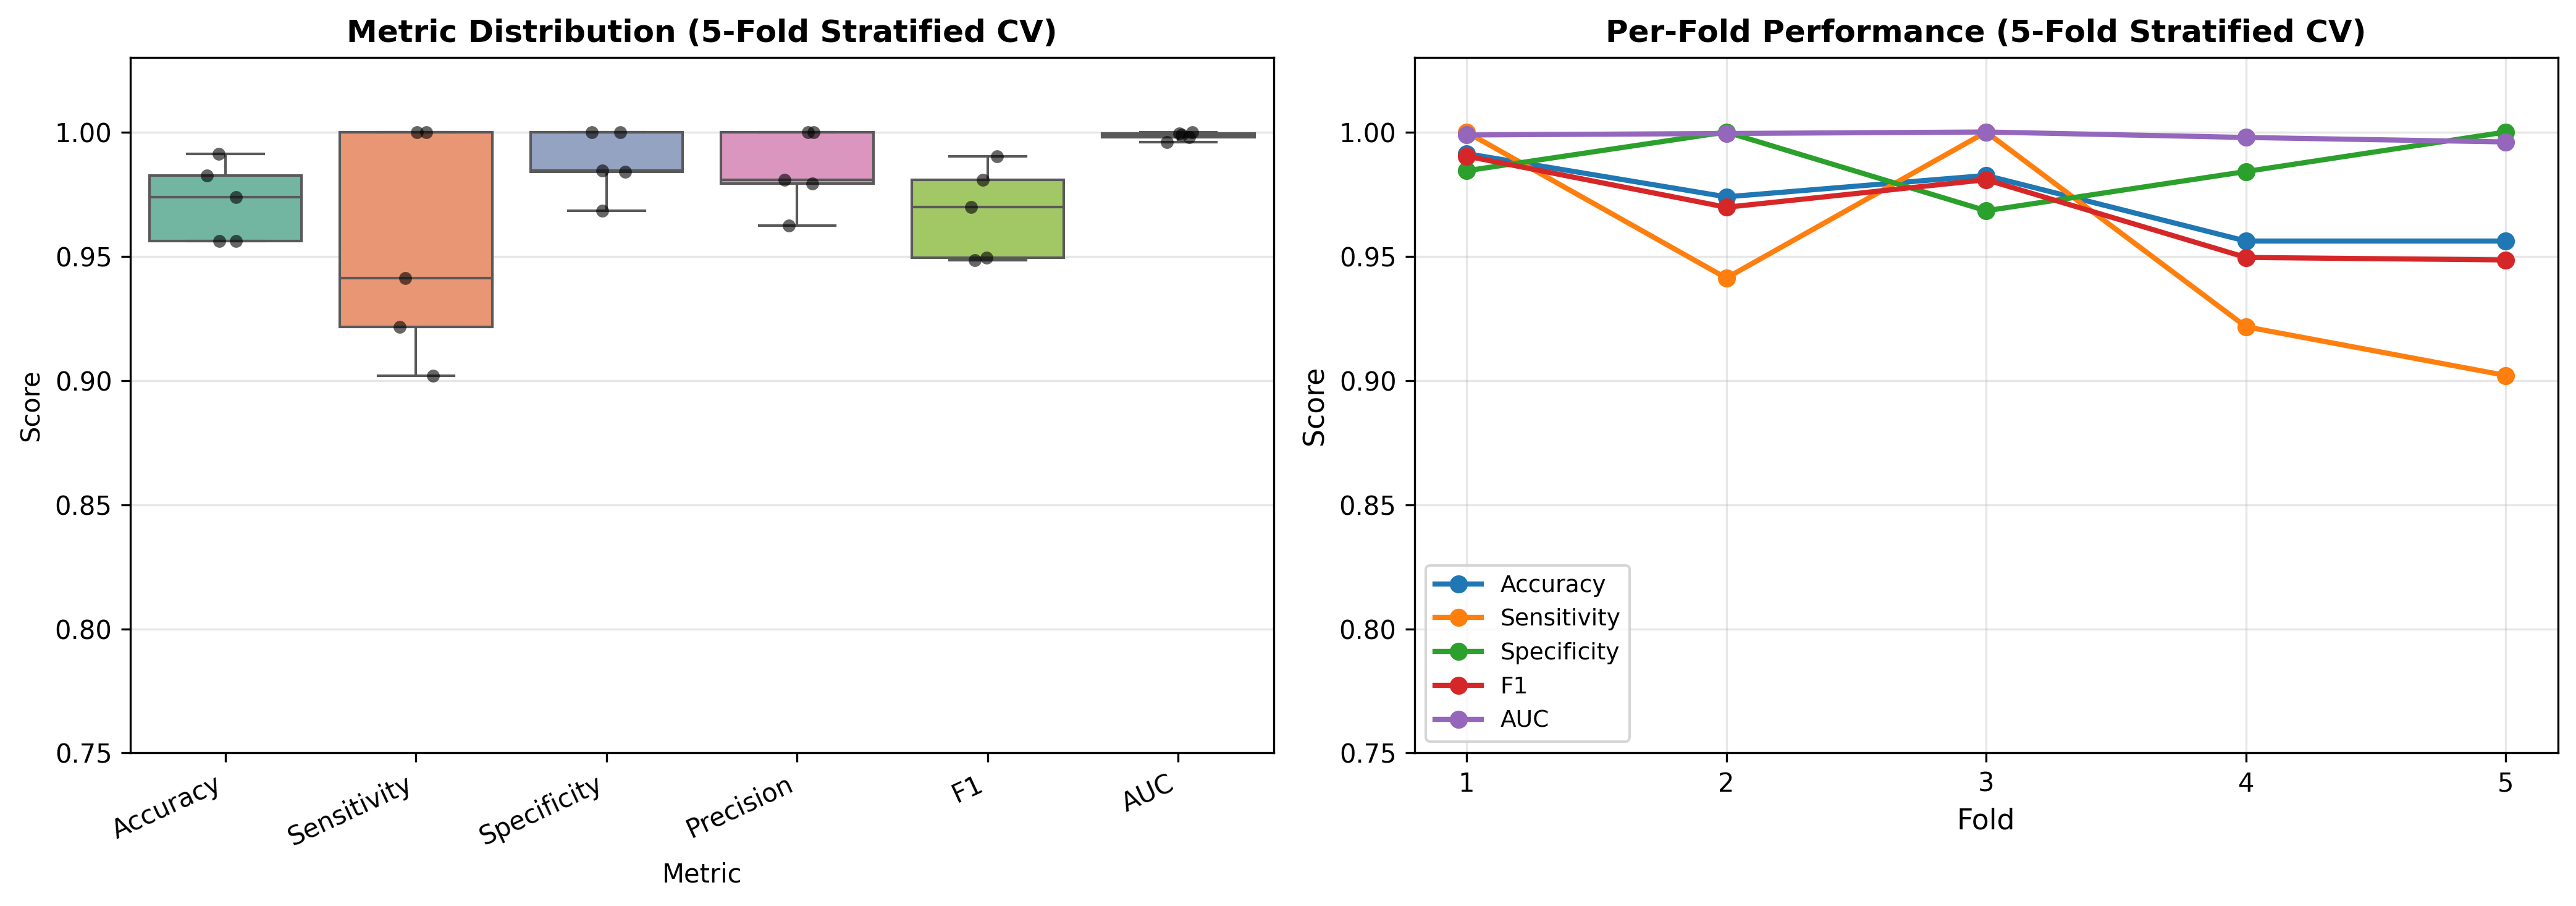
\includegraphics[width=0.98\textwidth]{figs/kfold_cv_metrics.png}
    \caption{Left: Boxplot distribution of classification metrics across the 5 stratified folds ($N=572$). Right: Per-fold metric trajectories.}
    \label{fig:kfold_cv}
\end{figure}

\begin{figure}[htbp]
    \centering
    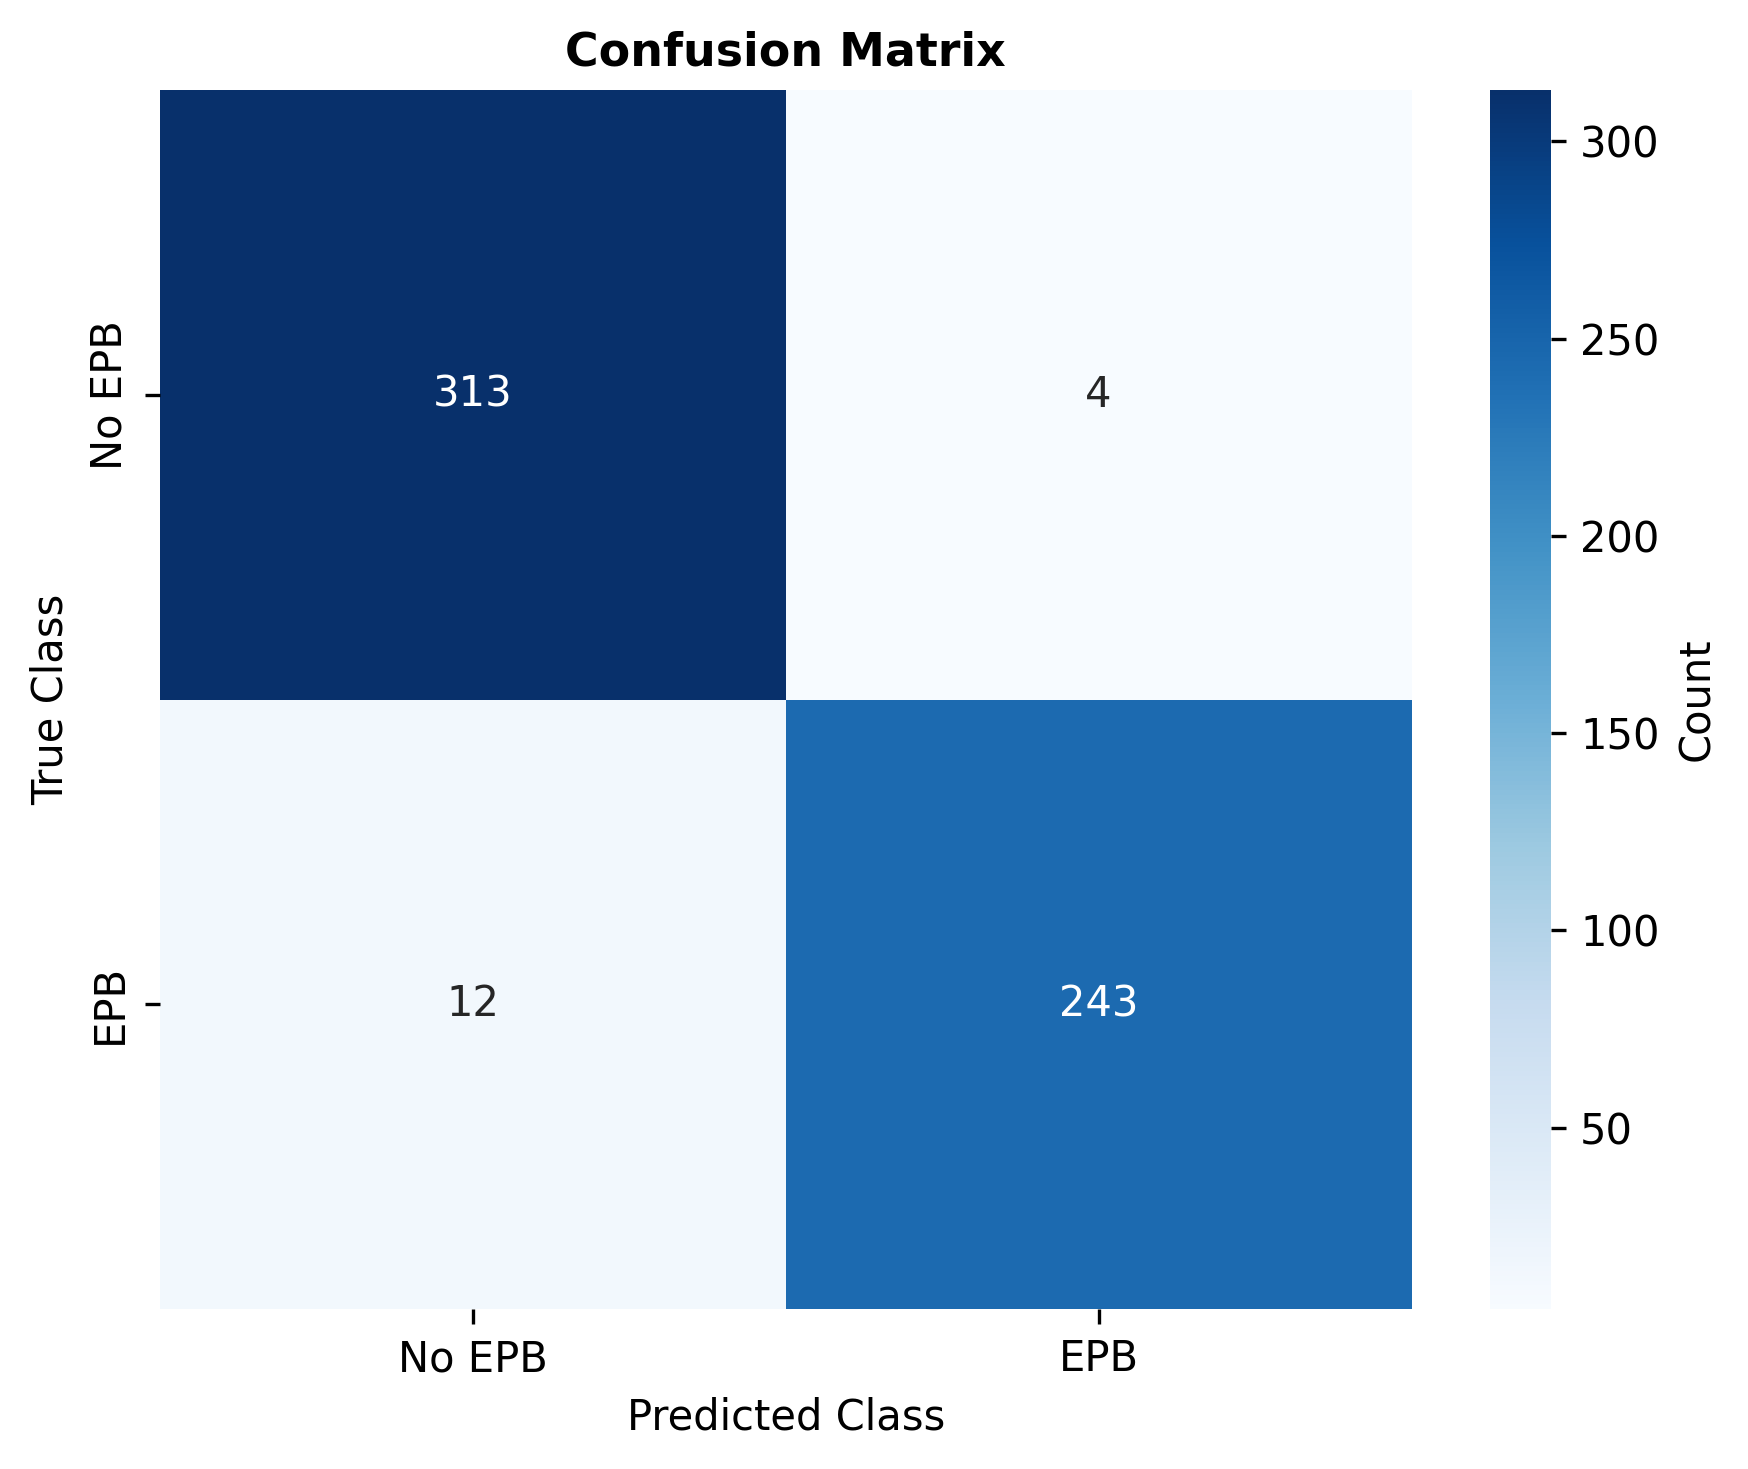
\includegraphics[width=0.52\textwidth]{figs/confusion_matrix.png}
    \caption{Out-of-fold confusion matrix aggregated across all $N=572$ labeled exposures ($313$ TN, $4$ FP, $12$ FN, $243$ TP).}
    \label{fig:confusion_matrix}
\end{figure}

\begin{figure}[htbp]
    \centering
    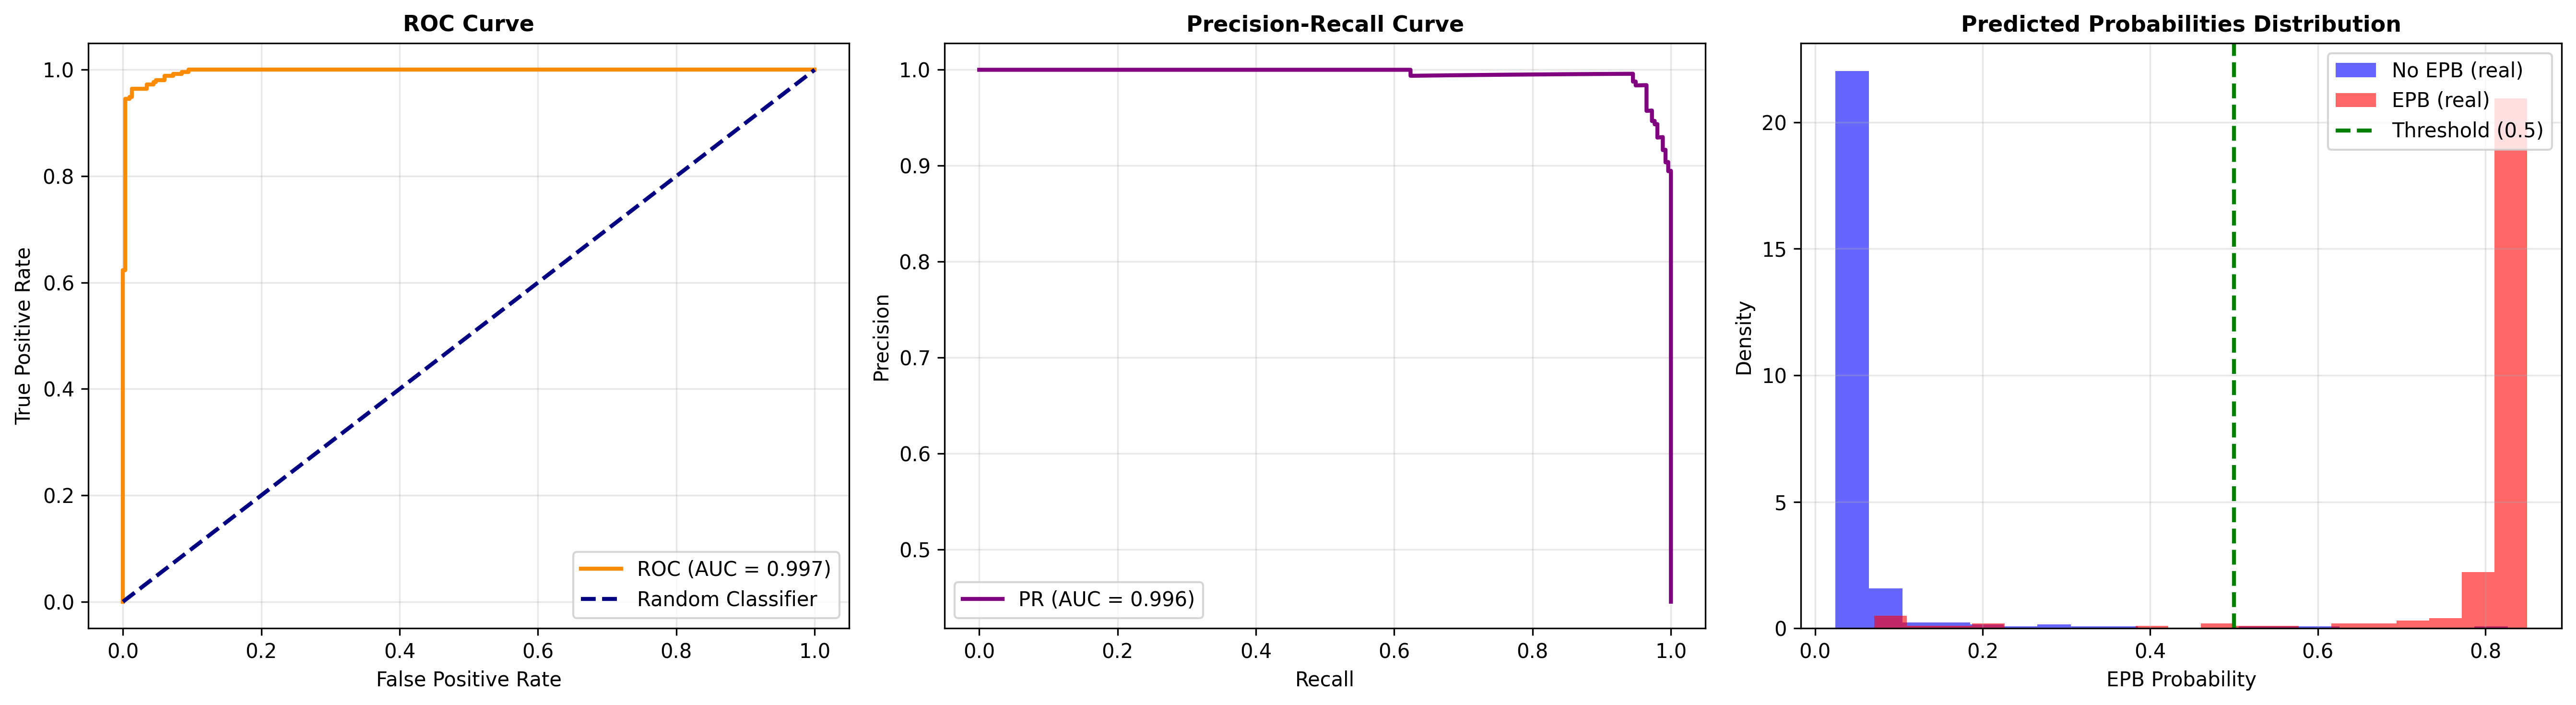
\includegraphics[width=0.98\textwidth]{figs/roc_pr_curves.png}
    \caption{Aggregated out-of-fold ROC curve (AUC $= 0.997$), Precision-Recall curve (AUC $= 0.996$), and predicted probability histogram across all $N=572$ labeled images.}
    \label{fig:roc_pr}
\end{figure}

Keeping each $30$-minute window inside a single fold lowered accuracy to $95.08\%$ and, above all, made sensitivity vary much more between folds ($90.88\% \pm 10.48\%$). This is expected: when a whole active window is held out, some depletion shapes are missing from training. ROC-AUC, however, stayed at $0.9969$ (PR-AUC $0.9978$), so the separation between classes does not depend on near-identical frames shared by training and validation. With the circular mask that hides the corner text, accuracy was $95.80\%$, about $1.4$ points below the unmasked model, and the holdout accuracy was unchanged ($96.50\%$). The classifier, therefore, does not rely on the printed annotations.

\subsection{Baselines, Ablations, and Shortcut Learning}

Table~\ref{tab:benchmark} and Figure~\ref{fig:benchmark} compare the pipeline with the baselines and ablations described in Section~\ref{sec:protocol}. Besides the holdout metrics, the table gives the zero-shot recall on CP (ZS-CP), which shows whether a good holdout score comes from the EPB structure or from cues tied to the station.

\begin{table}[htbp]
\centering
\caption{Baseline and ablation comparison on the stratified holdout test set ($n=143$), zero-shot recall on the unseen Cachoeira Paulista observatory (ZS-CP, $n=42$), and single-frame CPU inference latency.}
\label{tab:benchmark}
\resizebox{\textwidth}{!}{%
\setlength{\tabcolsep}{4pt}
\begin{tabular}{lcccccccc}
\toprule
\textbf{Model / Ablation Configuration} & \textbf{Acc} & \textbf{Sens} & \textbf{Spec} & \textbf{Prec} & \textbf{F1} & \textbf{ROC-AUC} & \textbf{ZS-CP} & \textbf{ms/img} \\
\midrule
Flatten ($4096$) + Logistic Regression & 0.9790 & 0.9688 & 0.9873 & 0.9841 & 0.9764 & 0.9992 & 0.9762 & 0.050 \\
1D-PCA ($320$) + Logistic Regression & 0.9860 & 1.0000 & 0.9747 & 0.9697 & 0.9846 & 0.9994 & 0.6905 & 0.070 \\
1D-PCA ($320$) + SVM (RBF) & 0.9510 & 1.0000 & 0.9114 & 0.9014 & 0.9481 & 0.9921 & 1.0000 & 0.231 \\
Flatten ($4096$) + Random Forest & 0.9720 & 1.0000 & 0.9494 & 0.9412 & 0.9697 & 0.9996 & 0.5476 & 0.678 \\
2DPCA ($k=5$) + SVM (RBF) & 0.9650 & 0.9688 & 0.9620 & 0.9538 & 0.9612 & 0.9978 & 1.0000 & 0.087 \\
2DPCA ($k=5$) + Random Forest & 0.9371 & 0.9062 & 0.9620 & 0.9508 & 0.9280 & 0.9909 & 1.0000 & 0.749 \\
2DPCA ($k=5$) + XGBoost & 0.9510 & 0.9375 & 0.9620 & 0.9524 & 0.9449 & 0.9958 & 1.0000 & 0.027 \\
2D-CNN (ConvNet Baseline) & 0.9720 & 1.0000 & 0.9494 & 0.9412 & 0.9697 & 0.9974 & 1.0000 & 0.769 \\
\midrule
Ablation: No Radiometric Preprocessing & 0.9930 & 1.0000 & 0.9873 & 0.9846 & 0.9922 & 1.0000 & 0.0000 & 0.570 \\
Ablation: No SMOTE Balancing & 0.9650 & 0.9531 & 0.9747 & 0.9683 & 0.9606 & 0.9970 & 1.0000 & 0.621 \\
Ablation: Circular FOV Mask & 0.9650 & 0.9531 & 0.9747 & 0.9683 & 0.9606 & 0.9964 & 1.0000 & 0.456 \\
2DPCA + Stacking Ensemble (Proposed) & 0.9650 & 0.9531 & 0.9747 & 0.9683 & 0.9606 & 0.9974 & 1.0000 & 0.630 \\
\bottomrule
\end{tabular}%
}
\end{table}

\begin{figure}[htbp]
    \centering
    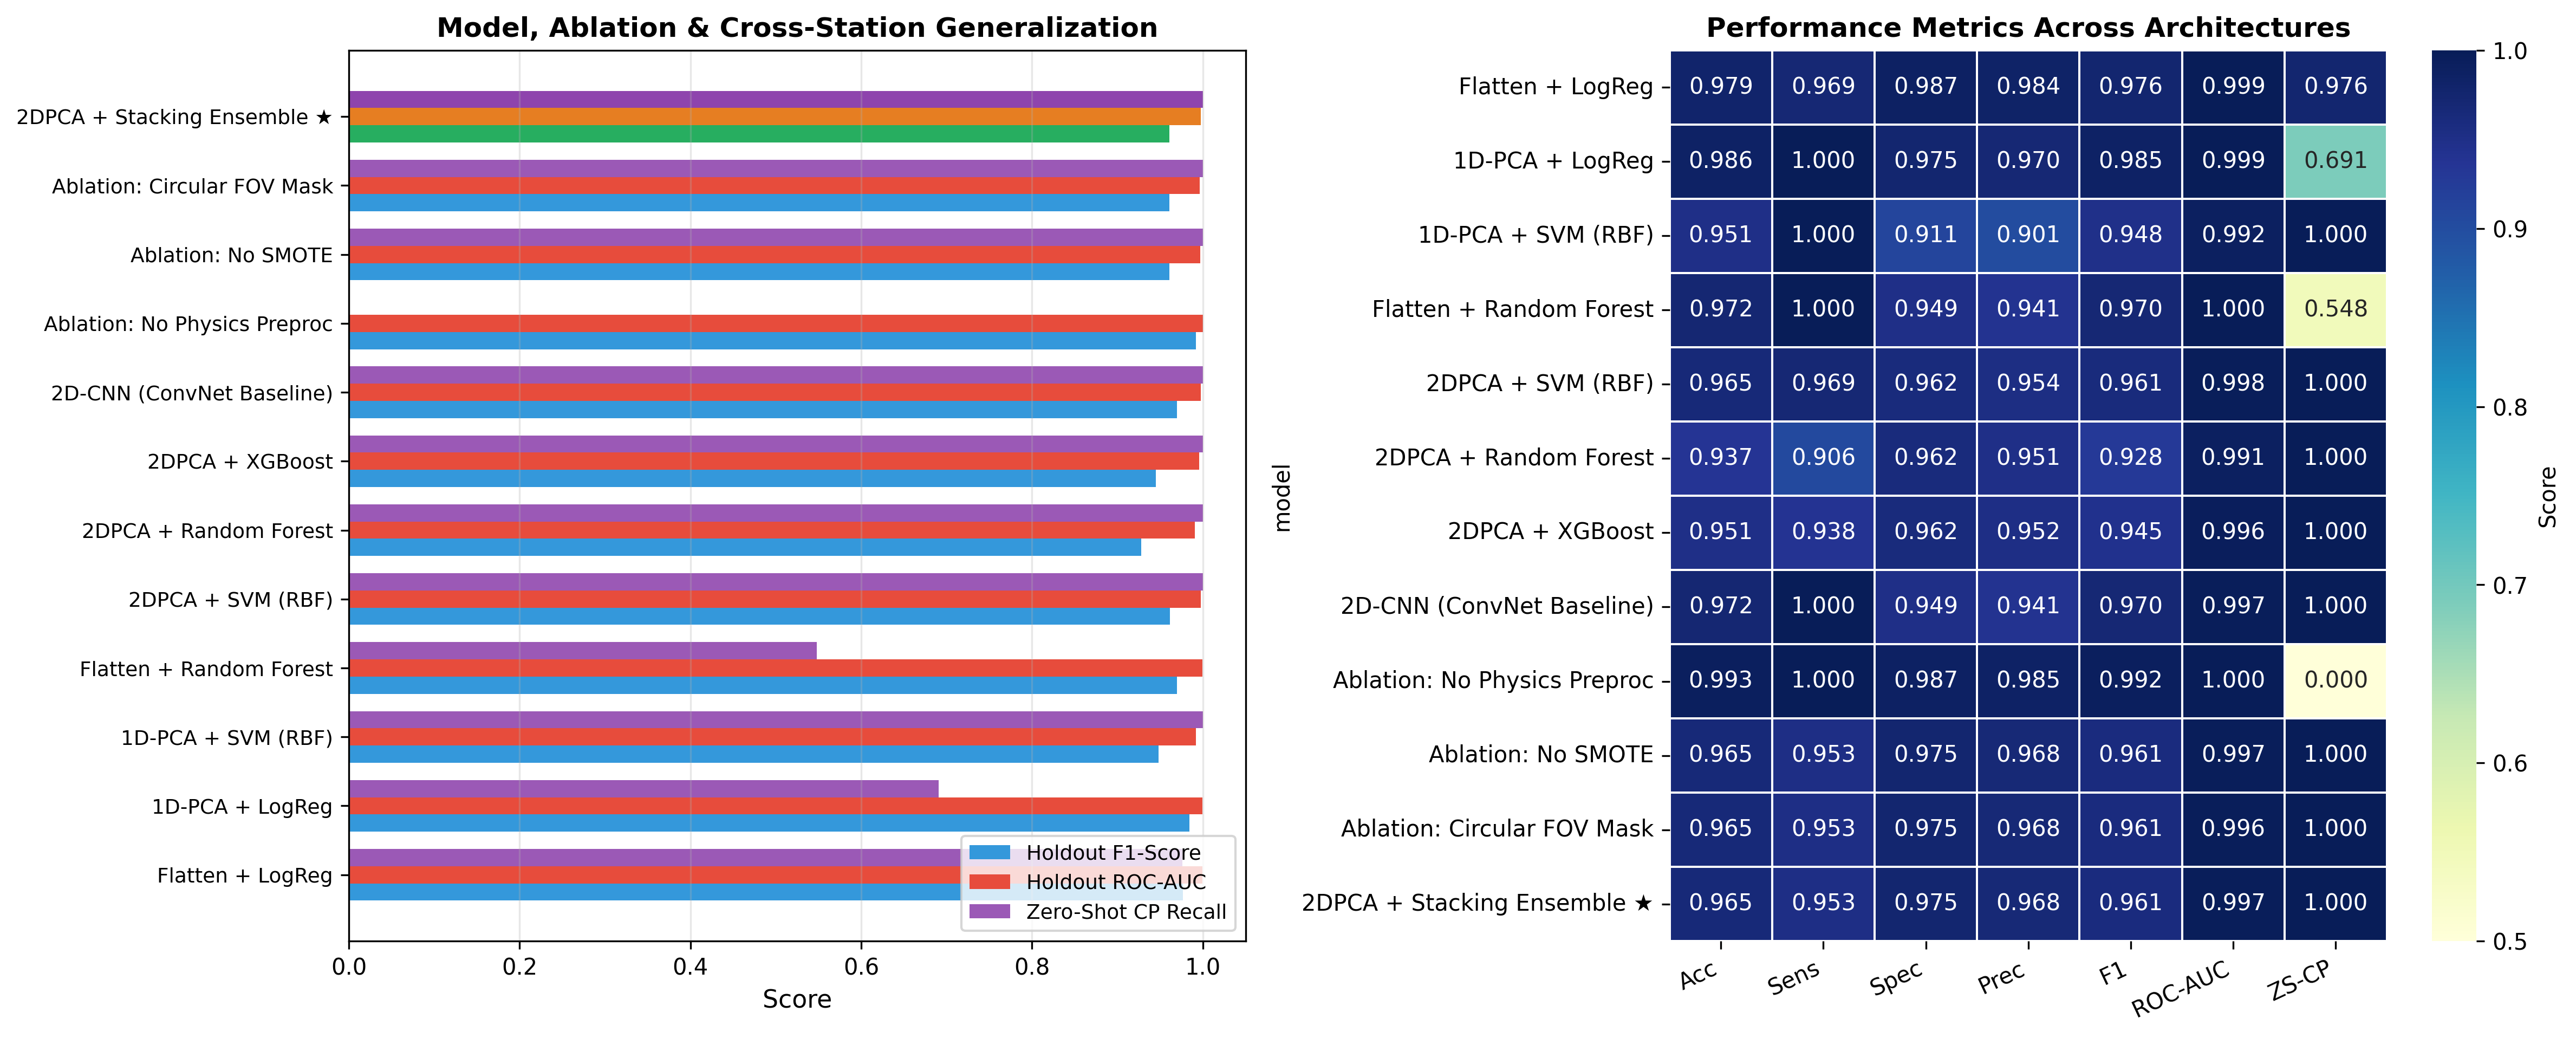
\includegraphics[width=0.98\textwidth]{figs/benchmark_baselines.png}
    \caption{Comparison of holdout F1-score, holdout ROC-AUC, and zero-shot Cachoeira Paulista recall (ZS-CP) across baselines, individual 2DPCA learners, 2D-CNN, and ablations.}
    \label{fig:benchmark}
\end{figure}

On the holdout split, the model without radiometric preprocessing had the best accuracy ($0.9930$), and the flattened and 1D-PCA models reached $0.9510$--$0.9860$. On CP, however, the model without preprocessing did not detect a single EPB ($0/42$). The most likely explanation is that, without background subtraction and CLAHE, it separated BJL (only negatives) from CA (mostly positives) by their overall brightness, a cue that does not hold at CP, whose background is brighter. Flatten + Random Forest and 1D-PCA + Logistic Regression also lost much of their recall at CP ($54.76\%$, $23/42$, and $69.05\%$, $29/42$), probably because they give weight to pixel positions tied to the geometry of each camera.

All models built on preprocessed 2DPCA features detected the $42$ EPB frames at CP, as did the 2D CNN and 1D-PCA + SVM. Within this group, the stacking ensemble had the highest specificity ($97.47\%$, against $96.20\%$ for each 2DPCA learner alone and $94.94\%$ for the CNN), with an inference time of $0.63\text{ ms}$ per image. Removing SMOTE did not change holdout accuracy ($0.9650$), which is expected given the mild $1.24:1$ class ratio, but it lowered the mean predicted probability on CP from $75.71\%$ to $68.50\%$. In-fold SMOTE thus makes the model more confident on the unseen station.

\subsection{Moonlight, Station Effects, and Cloud Screening}

Table~\ref{tab:hard_negatives} groups the operational tests. When the out-of-fold predictions are split by Moon illumination, accuracy is $97.47\%$ for images taken with less than $50\%$ illumination. On the $97$ bright-moon images (up to $99.6\%$ illumination), where glare saturates part of the dome, specificity is $95.88\%$: only four of these hard negatives were taken for EPBs, which suggests that the background subtraction removes most of the smooth glare gradient. By station, out-of-fold accuracy is $94.84\%$ at CA, which includes clear and partly cloudy periods, and $100\%$ at BJL and CP.

The full-night sequences show why Stage~1 is needed. Used alone, the Stage~2 classifier trained on clear skies raised a false alarm on $61$ of the $62$ frames of the overcast night \texttt{CA\_20260624}, because CLAHE turns dark cloud edges into high-contrast bands. With Stage~1, $49$ frames ($79.0\%$) were labeled \texttt{CLOUDY} and $7$ ($11.3\%$) \texttt{DEGRADED}, and false alarms fell from $61$ to $13$ ($-78.7\%$), or to $6$ ($-90.2\%$) if alerts are issued only for \texttt{CLEAR} frames. On the clear night \texttt{BJL\_20250722}, Stage~1 blocked $14$ twilight or hazy frames ($6.1\%$) and, with them, the $3$ false alarms produced by Stage~2 alone. On the active night \texttt{CA\_20251022}, only $4$ frames ($2.9\%$) were flagged as cloudy, and $125$ EPB detections were kept ($89.3\%$ of the frames, $122$ of them under \texttt{CLEAR} sky).

\begin{table}[htbp]
\centering
\caption{Operational evaluation across lunar illumination regimes, observatory sites (including zero-shot transfer to CP), and continuous nocturnal sequences comparing Stage~2 alone (trained on clear skies, $n=510$) against the two-stage cascaded pipeline.}
\label{tab:hard_negatives}
\resizebox{\textwidth}{!}{%
\setlength{\tabcolsep}{4.5pt}
\begin{tabular}{llcccc}
\toprule
\textbf{Evaluation Scenario} & \textbf{Protocol / Mode} & \textbf{Frames} & \textbf{QC Flagged} & \textbf{Metric / Result} \\
\midrule
Low/Moderate Moon ($<50\%$) & 5-Fold OOF & 475 & -- & Acc: $97.47\%$ / Spec: $100.0\%$ ($220/220$) \\
Bright Lunar Glare ($\ge 50\%$) & 5-Fold OOF (Hard Neg.) & 97 & -- & Specificity: $95.88\%$ ($93/97$) \\
\midrule
São João do Cariri (CA) & 5-Fold OOF & 310 & -- & Accuracy: $94.84\%$ \\
Bom Jesus da Lapa (BJL) & 5-Fold OOF & 220 & -- & Specificity: $100.0\%$ ($220/220$) \\
Cachoeira Paulista (CP) & Zero-Shot (Train: CA+BJL) & 42 & -- & Recall: $100.0\%$ ($42/42$) \\
\midrule
\texttt{BJL\_20250722} (Clear Quiet) & Stage 2 Only vs. Cascaded & 230 & $14$ ($6.1\%$) & FP: $3 \to 0$ ($100.0\%$ Spec.) \\
\texttt{CA\_20260624} (Overcast Sky) & Stage 2 Only vs. Cascaded & 62 & $49$ ($79.0\%$) & FP: $61 \to 13$ ($6$ Clear, $-78.7\%$ / $-90.2\%$) \\
\texttt{CA\_20251022} (Active EPB) & Stage 2 Only vs. Cascaded & 140 & $4$ ($2.9\%$) & Valid EPB: $125$ ($89.3\%$) \\
\bottomrule
\end{tabular}%
}
\end{table}

\subsection{SHAP Attribution and Full-Night Time Series}

Figures~\ref{fig:shap_without} and~\ref{fig:shap_with} show the SHAP values mapped back to pixel space (Section~\ref{sec:model}) for the same quiet and active frames used in Figures~\ref{fig:recon_error_without} and~\ref{fig:recon_error_with}.

\begin{figure}[htbp]
    \centering
    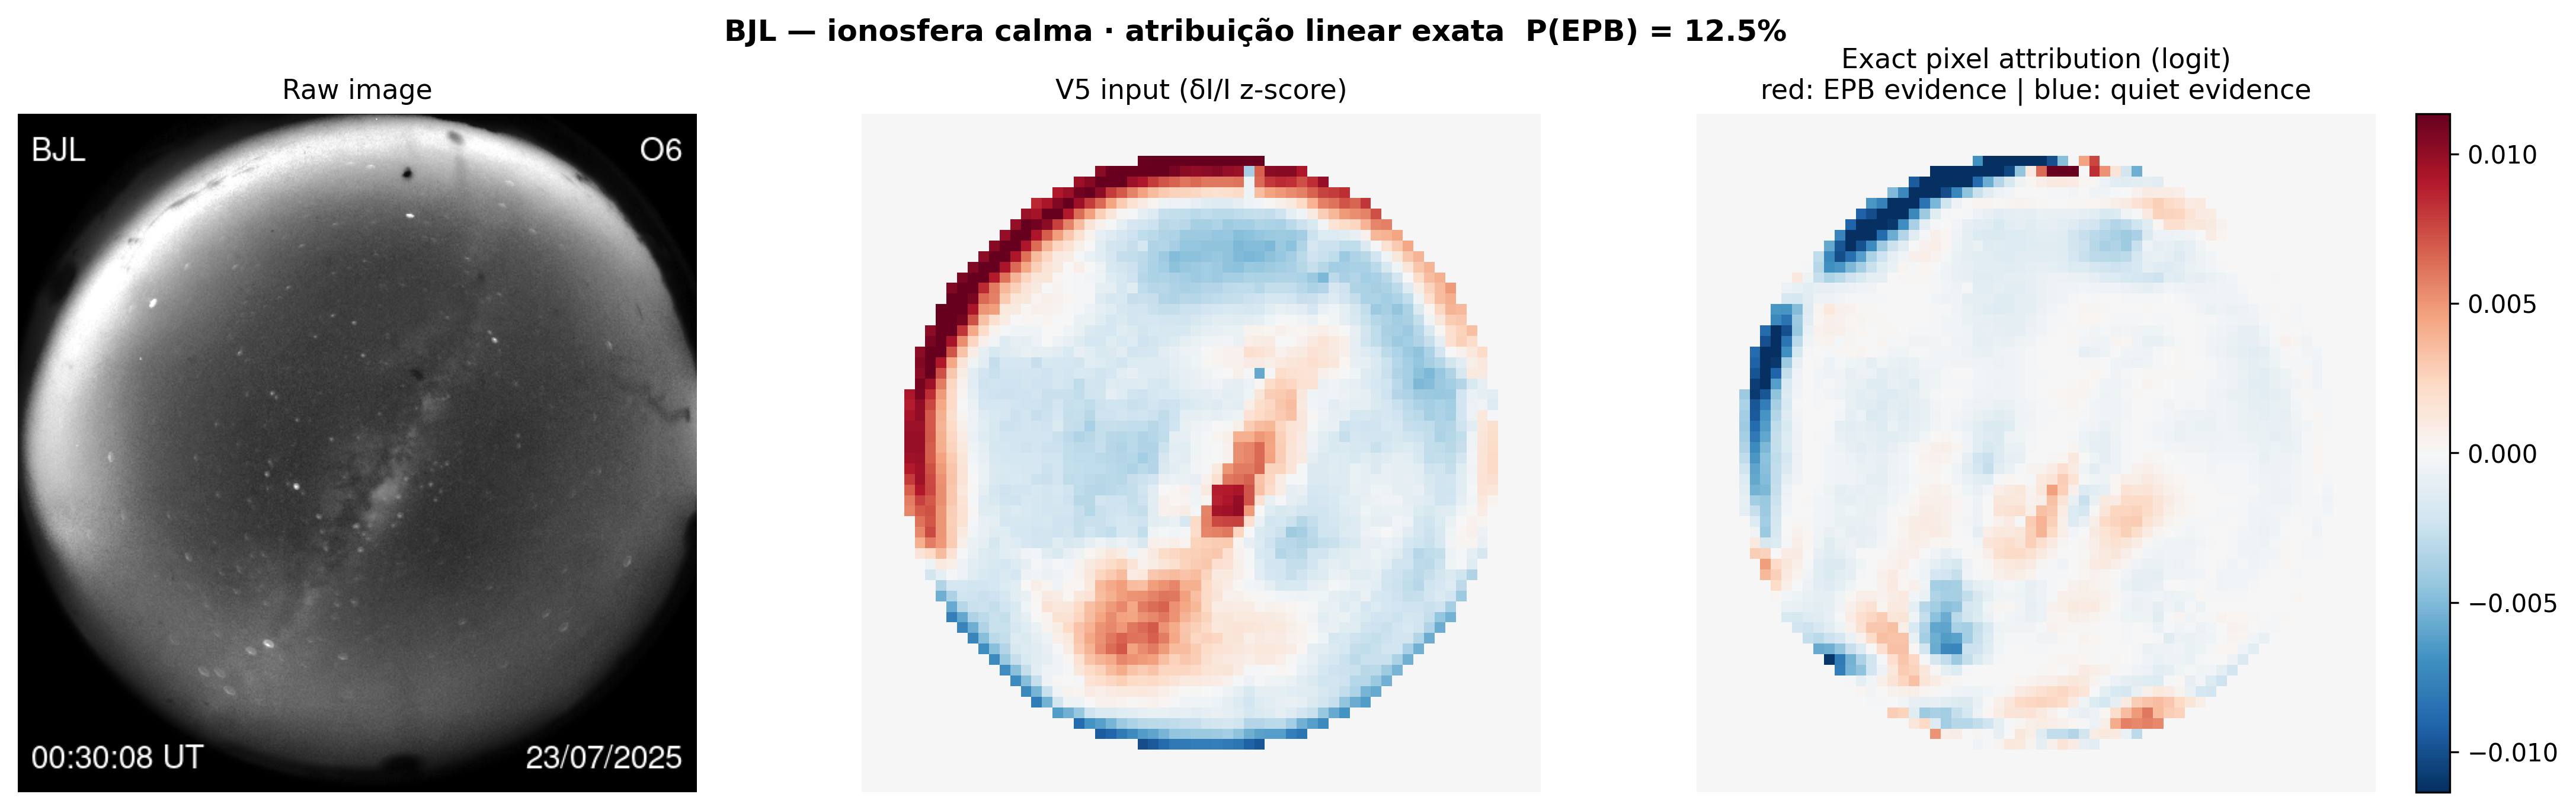
\includegraphics[width=0.98\textwidth]{figs/shap_analysis_without.png}
    \caption{Pixel-space SHAP attribution for a quiet-sky exposure from Bom Jesus da Lapa (True: No EPB, Predicted: No EPB, $0.4\%$). Blue regions denote negative attributions that reduce EPB probability.}
    \label{fig:shap_without}
\end{figure}

\begin{figure}[htbp]
    \centering
    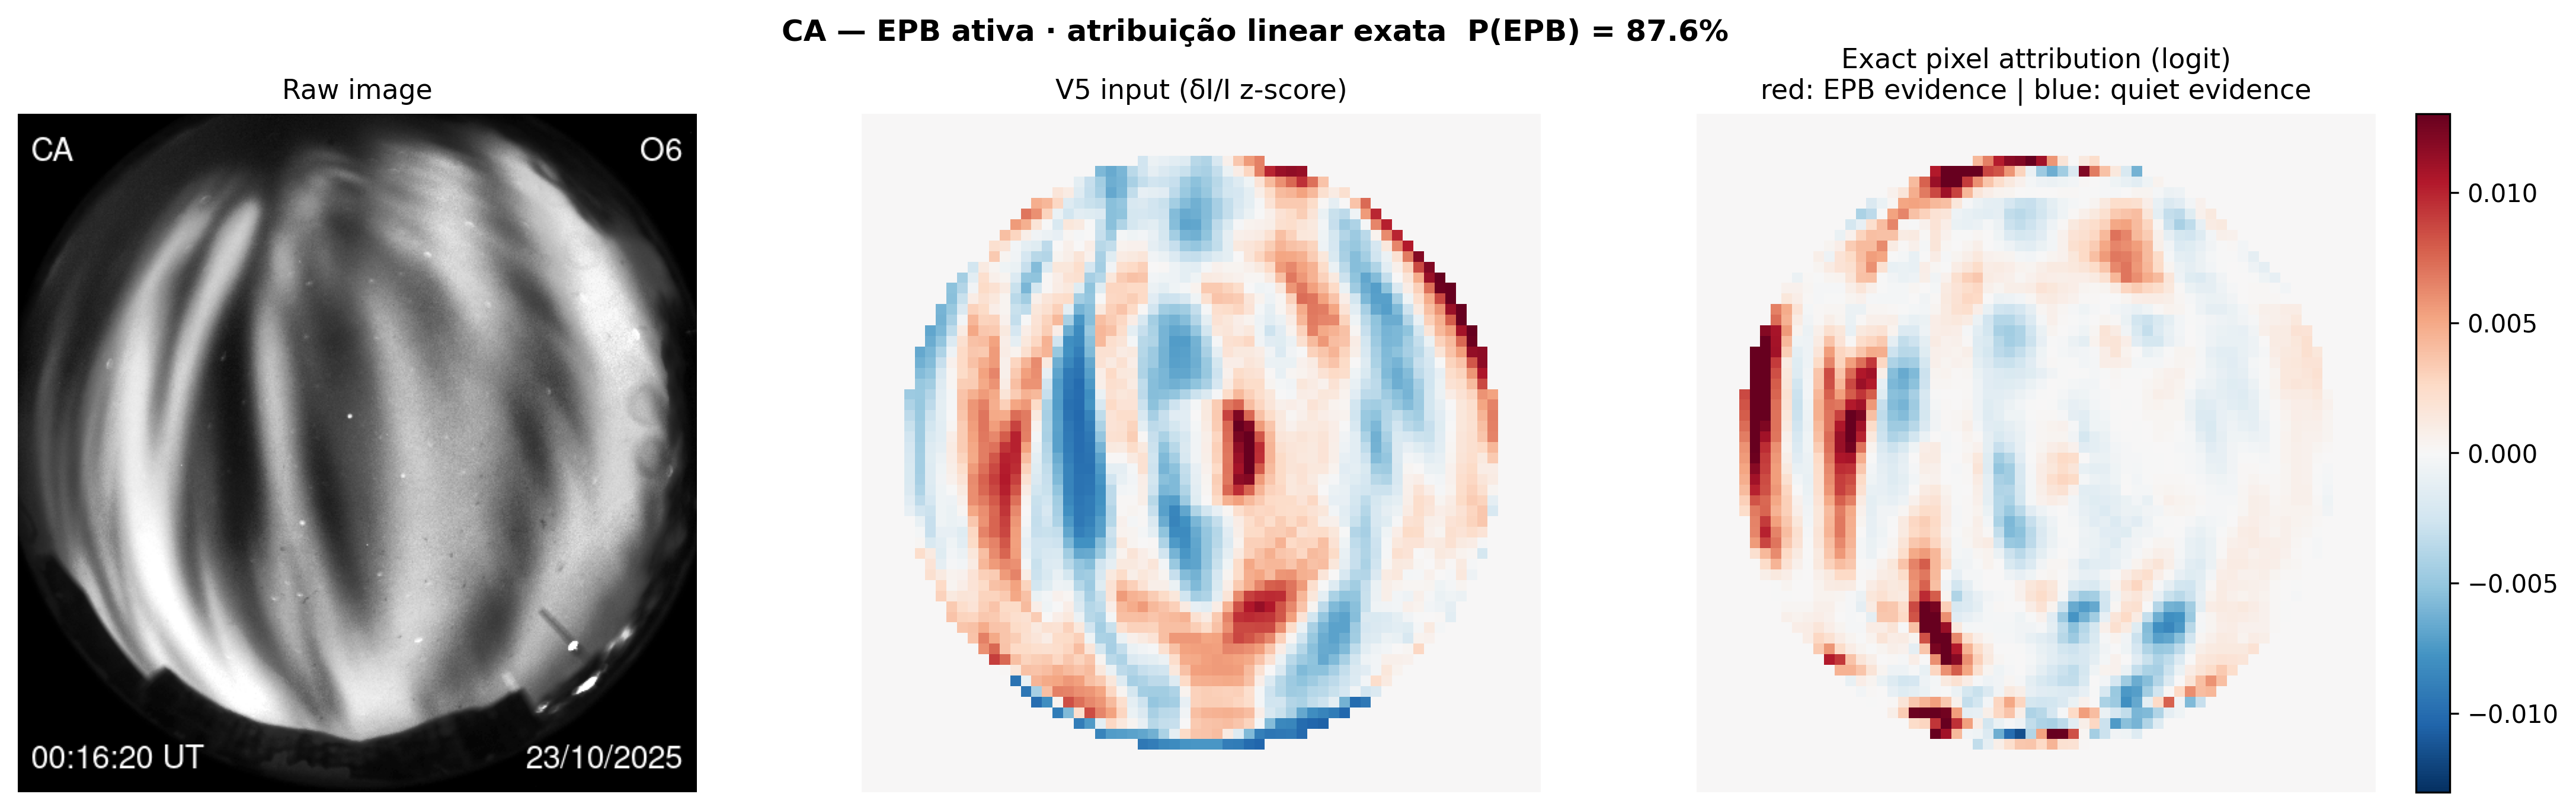
\includegraphics[width=0.98\textwidth]{figs/shap_analysis_with.png}
    \caption{Pixel-space SHAP attribution for an active EPB exposure from Cariri (True: EPB, Predicted: EPB, $99.2\%$). Red bands mark positive attributions aligned with the plasma depletion channels.}
    \label{fig:shap_with}
\end{figure}

In the quiet frame, negative values cover the center of the dome and keep the EPB probability at $0.4\%$. In the active frame ($99.2\%$), positive values follow the dark north--south depletion bands, and the four corners with text receive almost no attribution.

\begin{figure}[htbp]
    \centering
    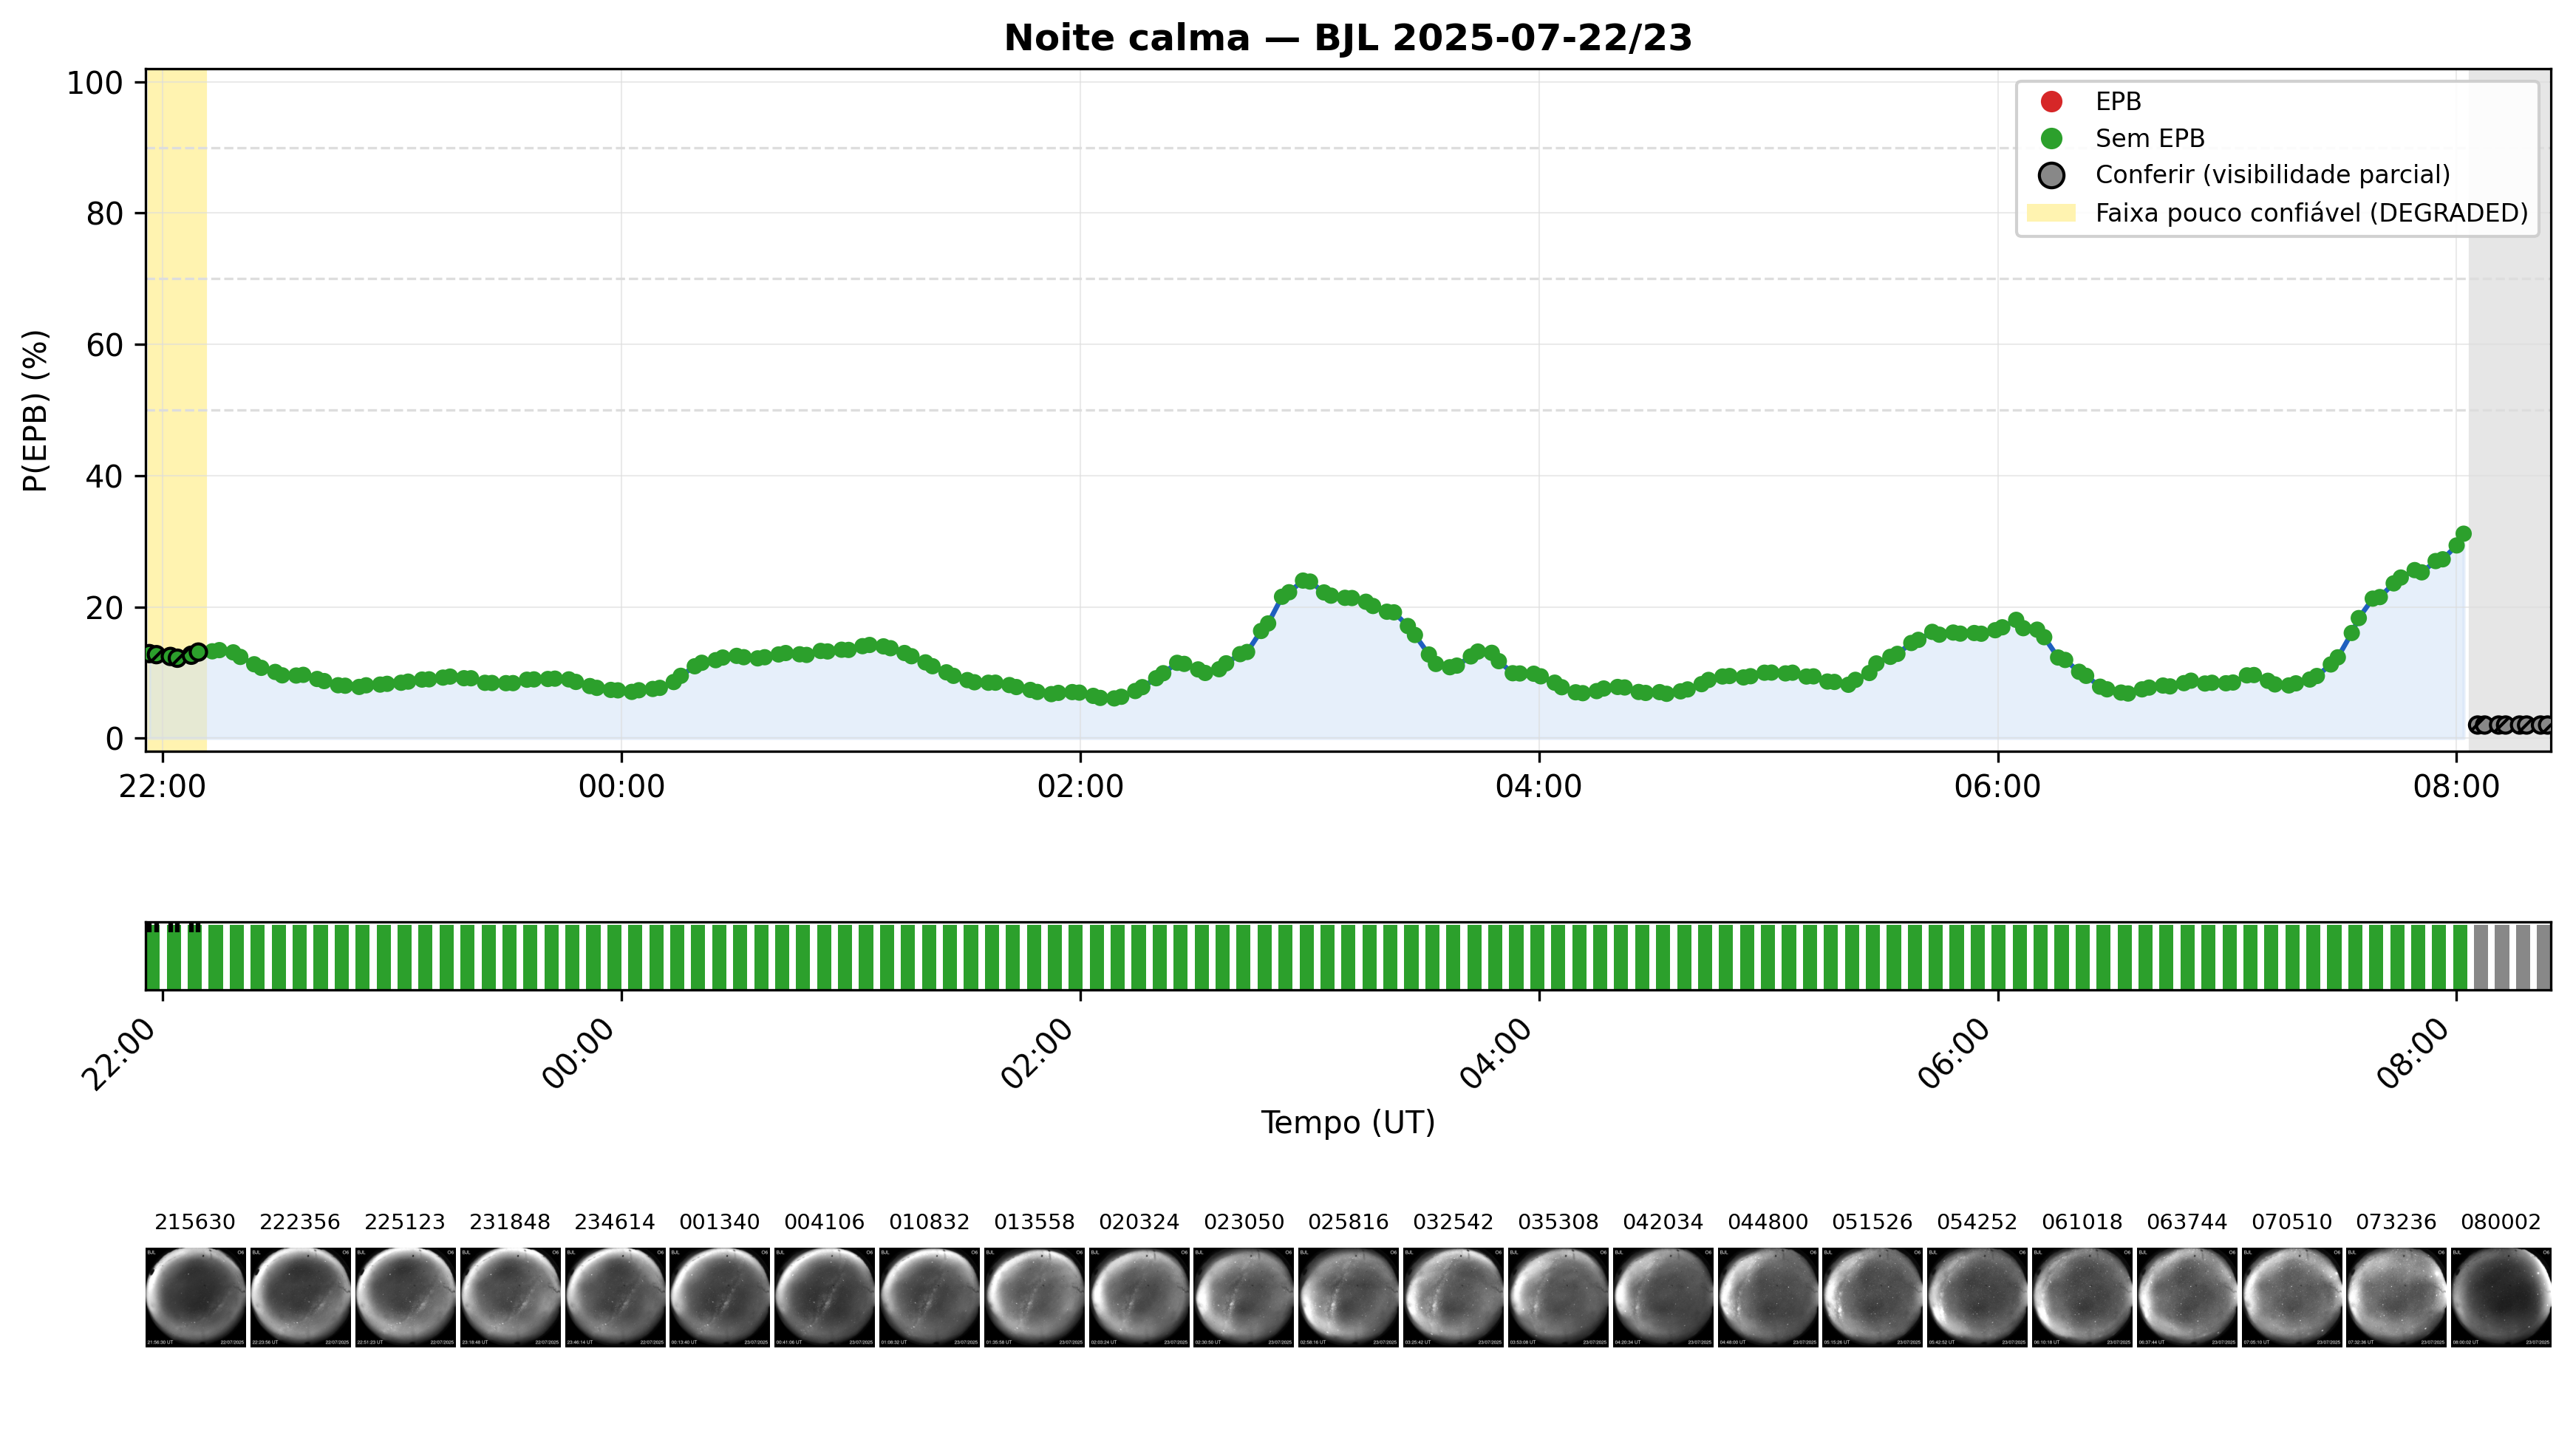
\includegraphics[width=0.98\textwidth]{figs/temporal_without_epb.png}
    \caption{Nocturnal time series on a clear quiet night at Bom Jesus da Lapa (\texttt{BJL\_20250722}, $230$ exposures). Predicted EPB probabilities remain near $0.4\%$ all night ($0$ false alarms).}
    \label{fig:temporal_without}
\end{figure}

\begin{figure}[htbp]
    \centering
    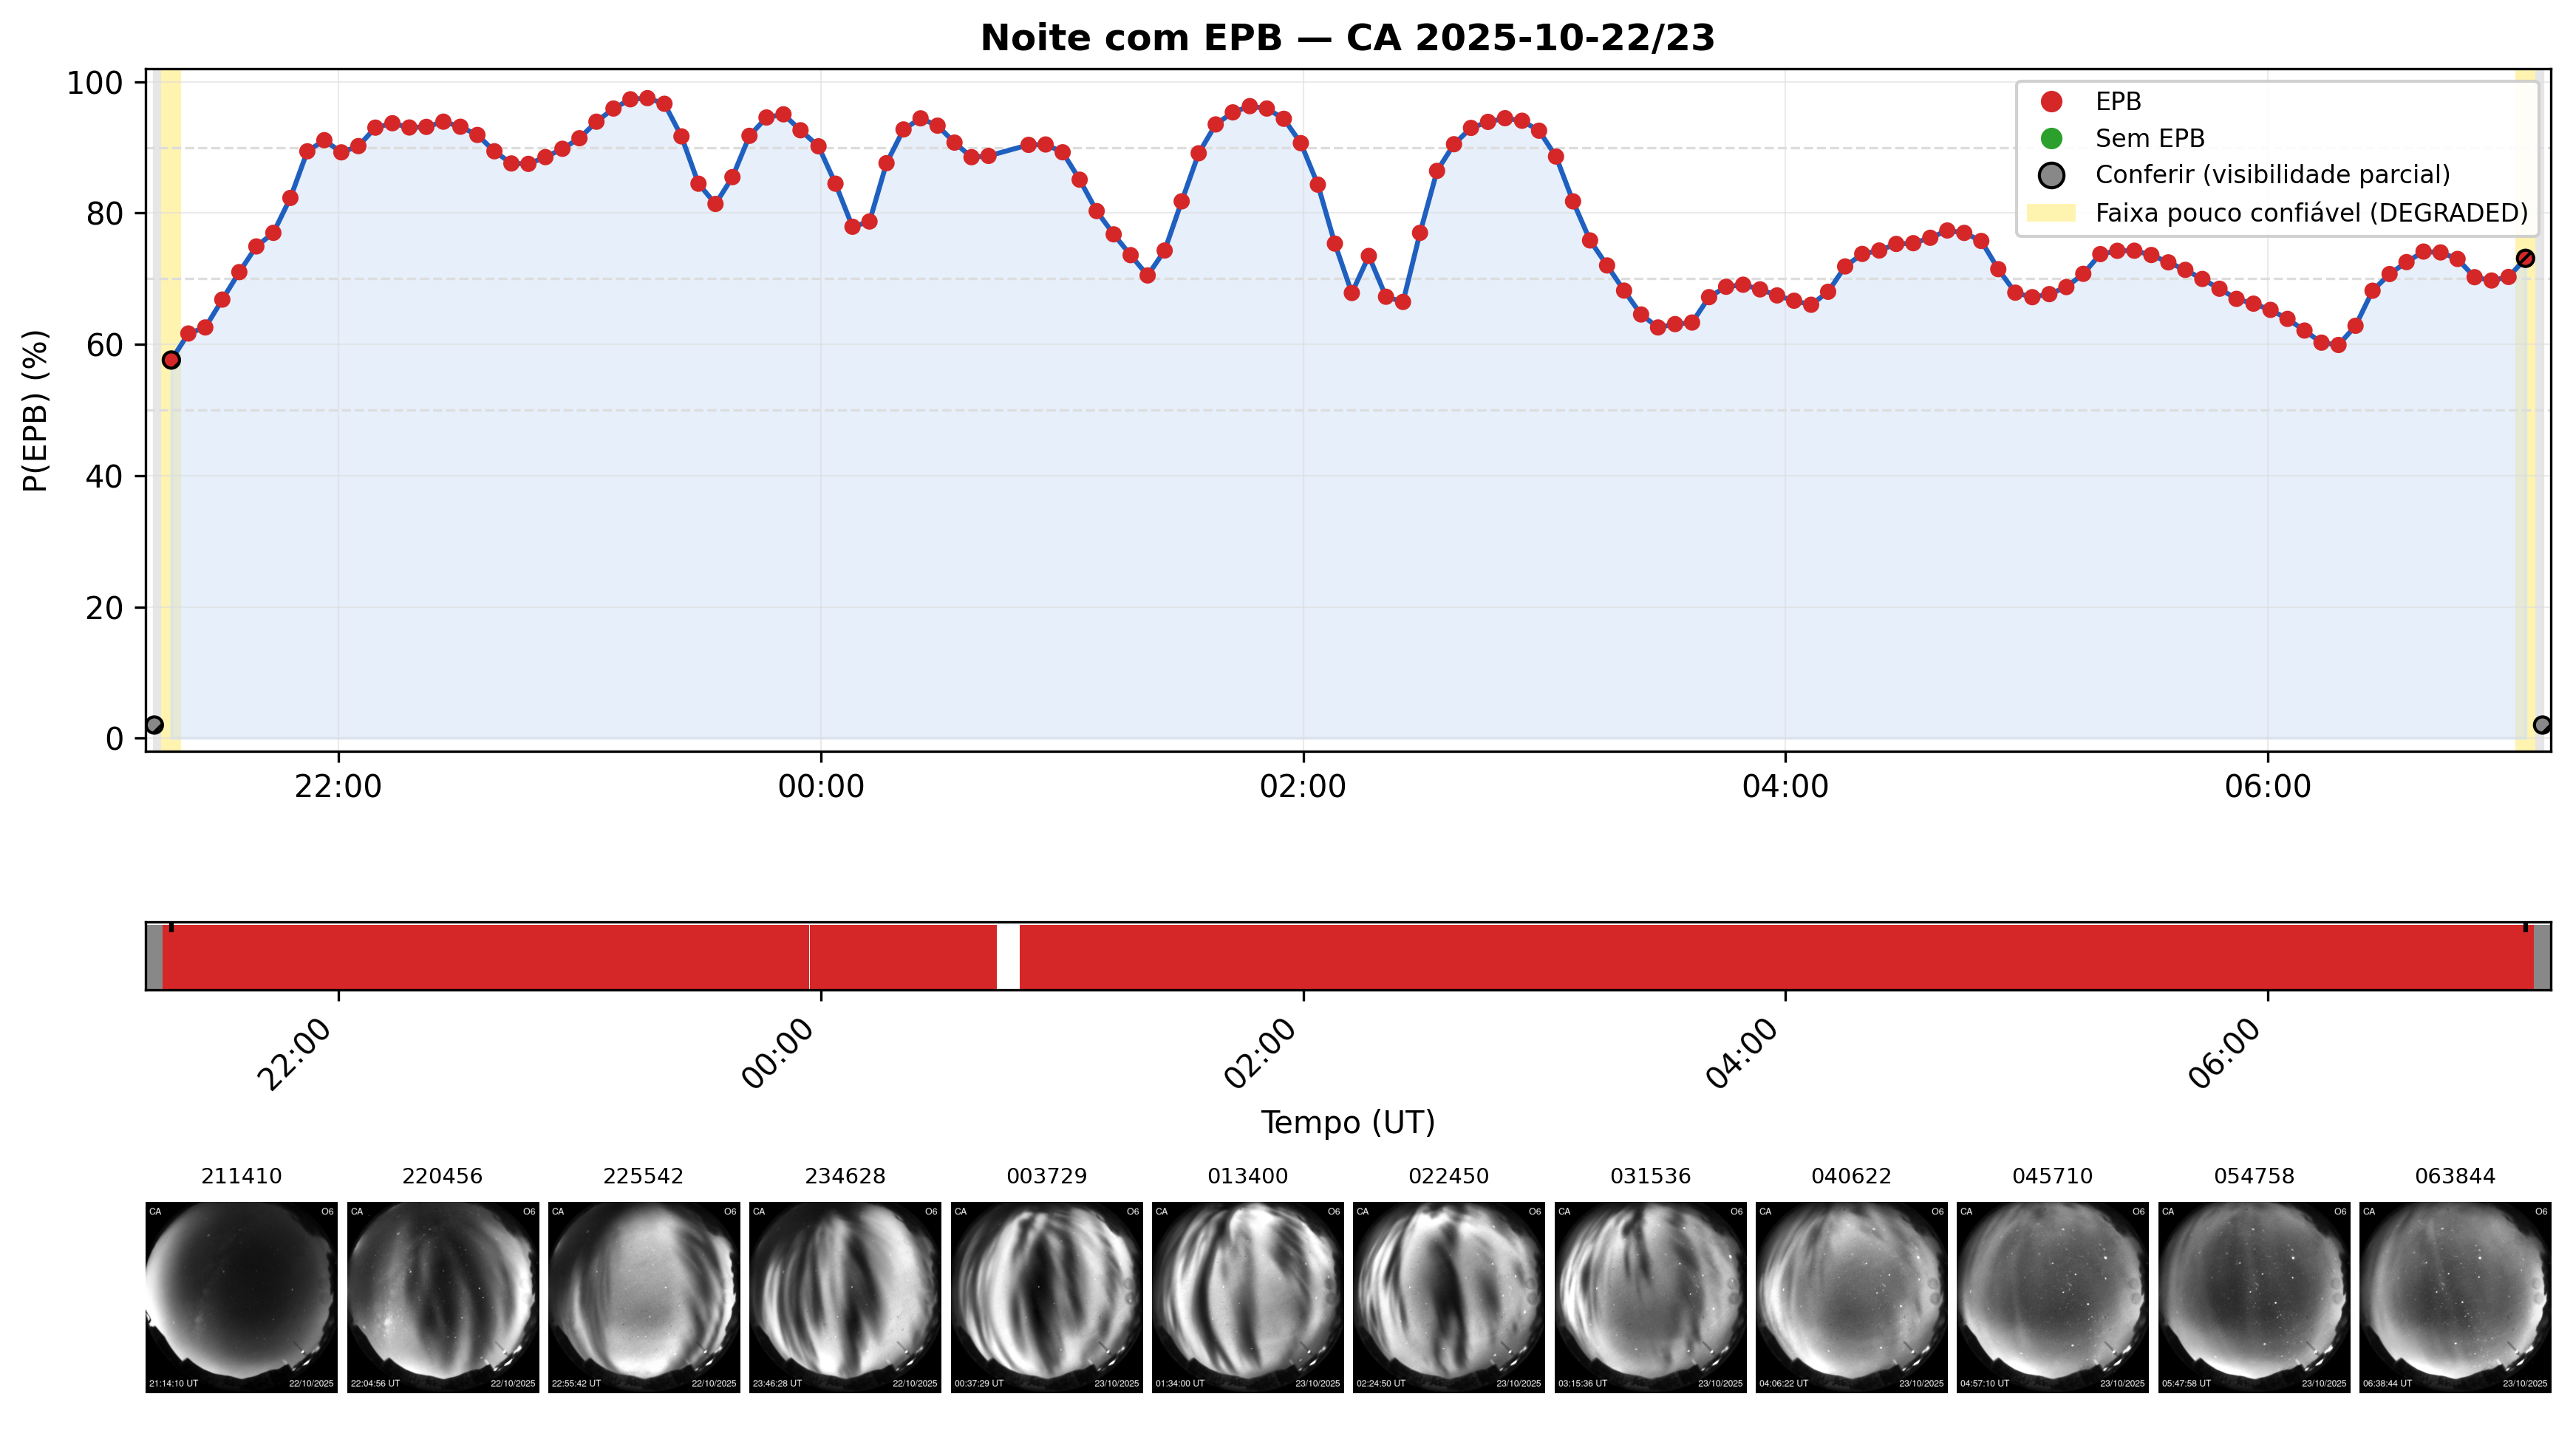
\includegraphics[width=0.98\textwidth]{figs/temporal_with_epb.png}
    \caption{Nocturnal time series on an active EPB night at Cariri (\texttt{CA\_20251022}, $140$ exposures), capturing bubble onset after $21{:}18\text{ UT}$, sustained zenith passage ($138/140$ frames), and pre-dawn decay.}
    \label{fig:temporal_with}
\end{figure}

\begin{figure}[htbp]
    \centering
    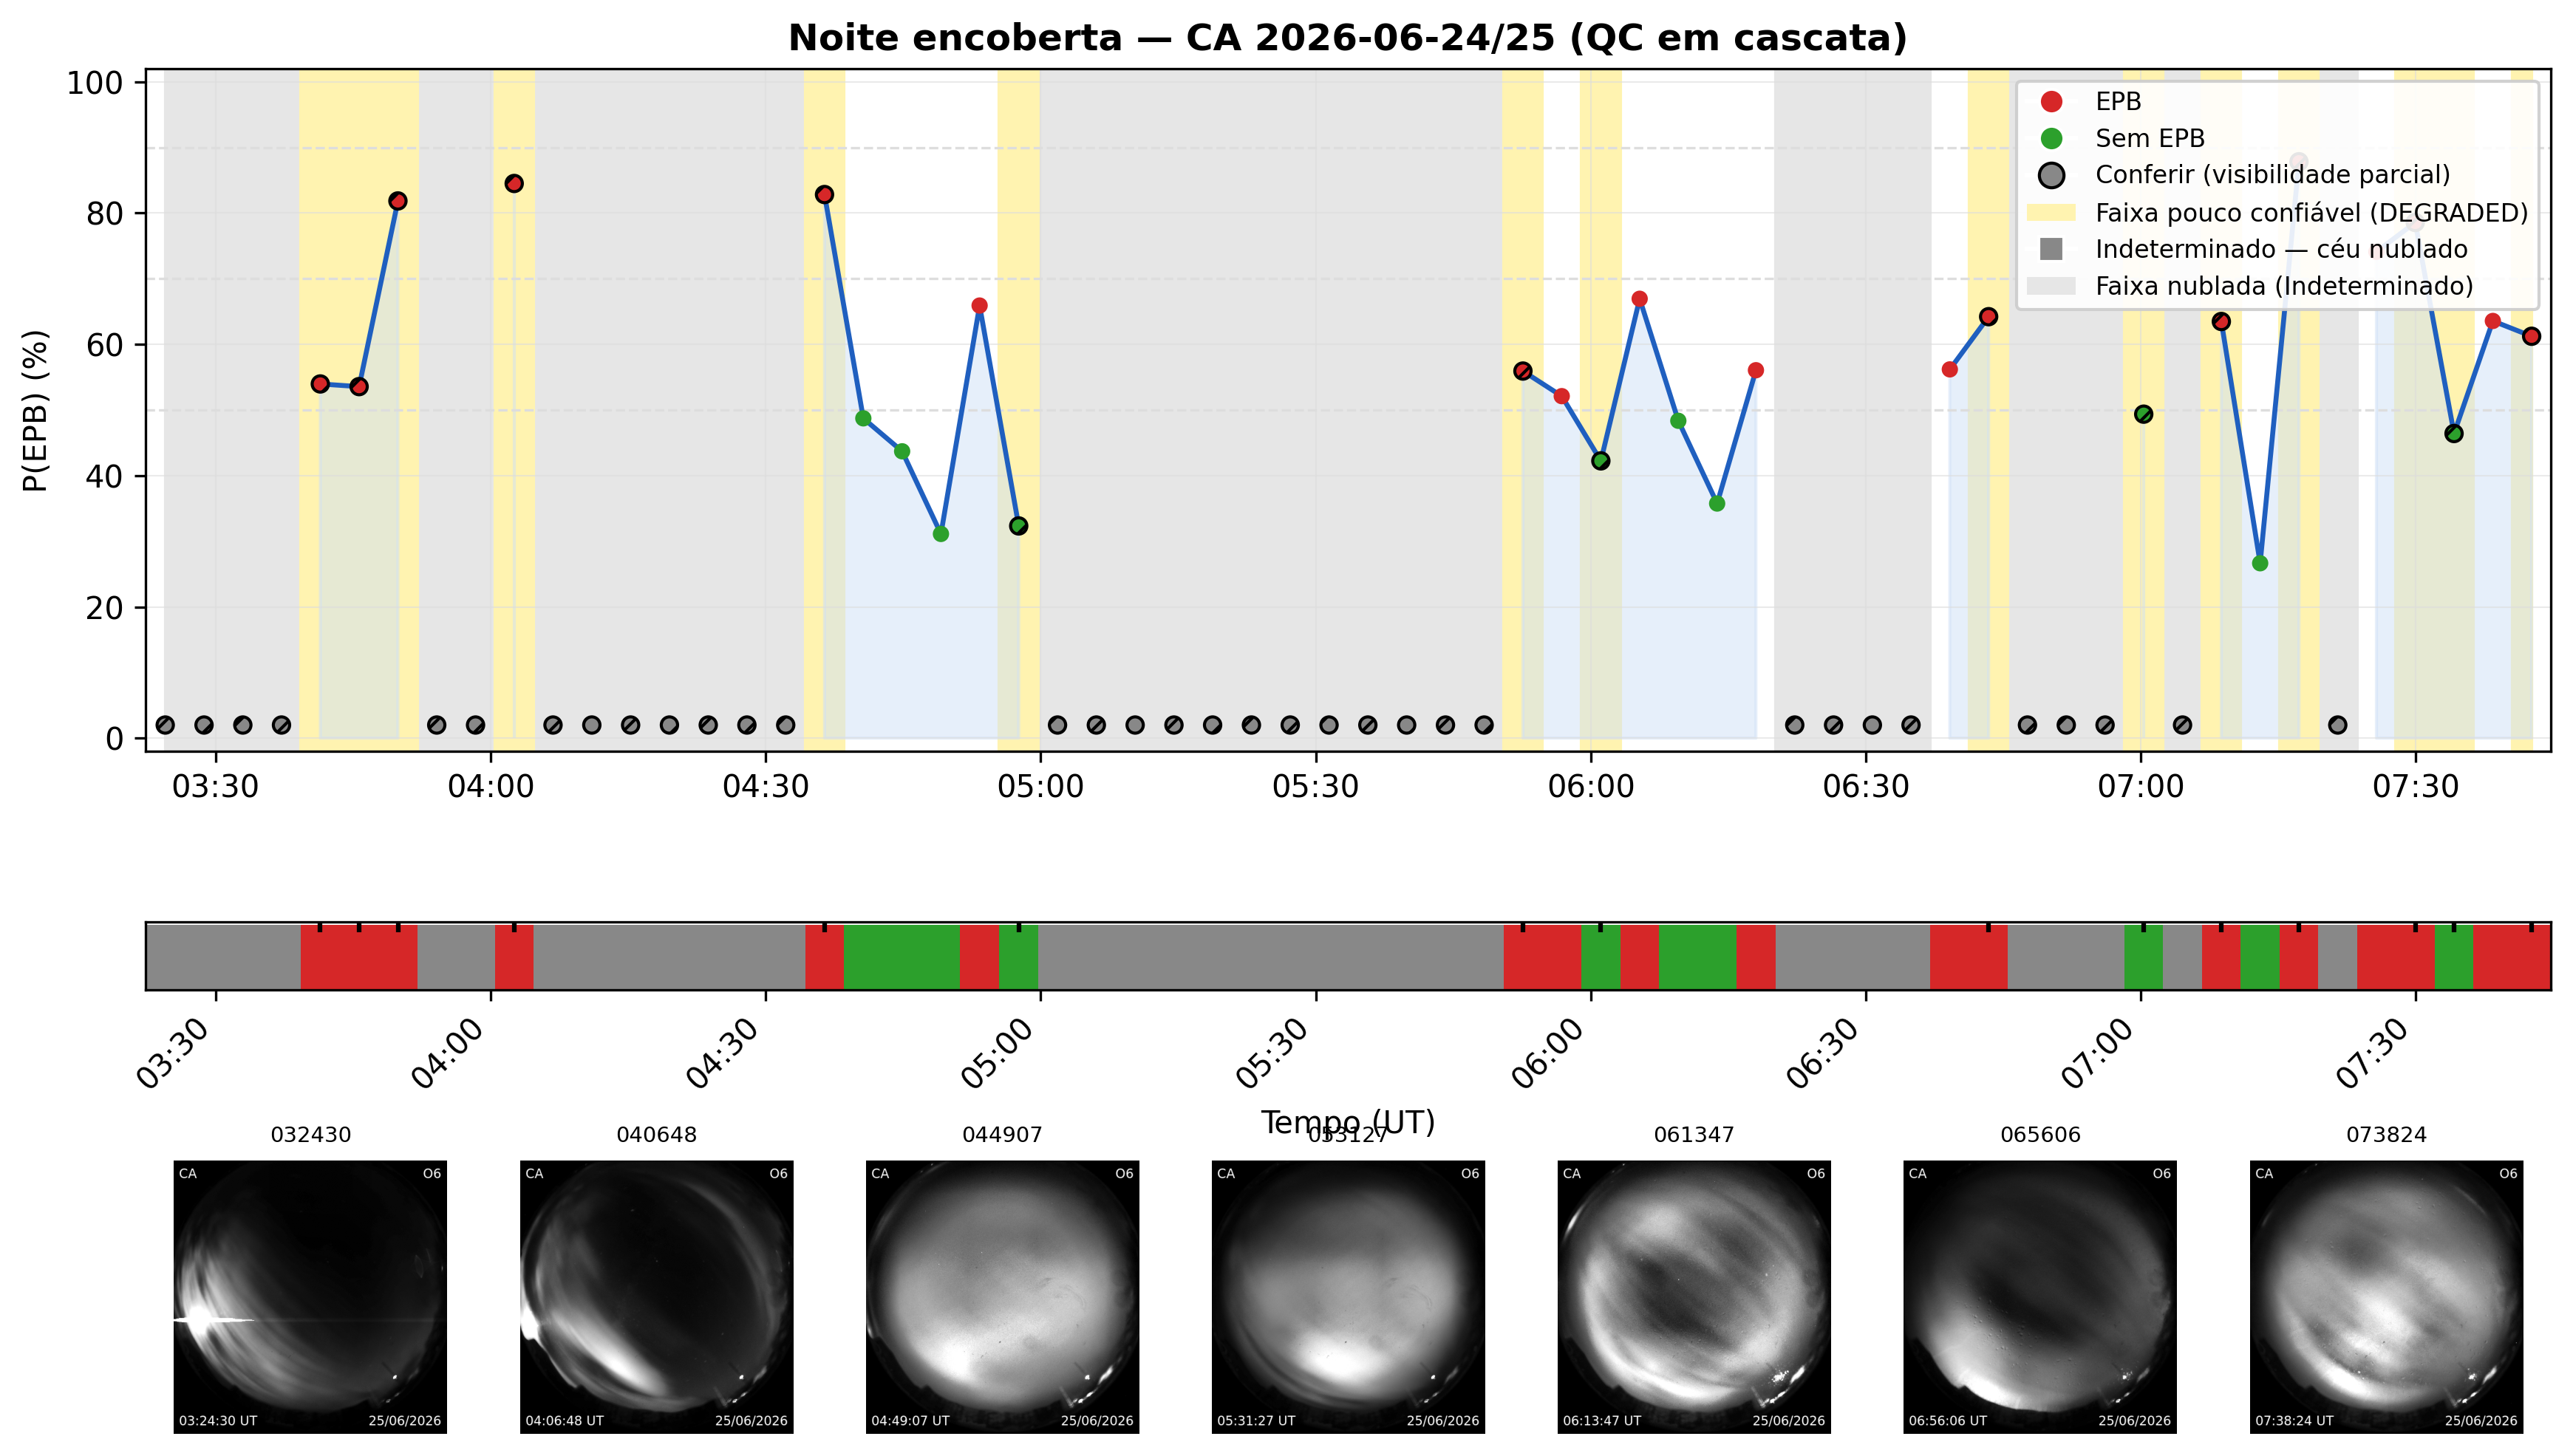
\includegraphics[width=0.98\textwidth]{figs/temporal_cloudy_qc.png}
    \caption{Cascaded nocturnal monitoring on an overcast night at Cariri (\texttt{CA\_20260624}, $62$ exposures). Stage~1 Sky QC (gray status intervals) flags $49/62$ frames ($79.0\%$) as cloudy.}
    \label{fig:temporal_cloudy}
\end{figure}

Figures~\ref{fig:temporal_without}--\ref{fig:temporal_cloudy} show the output of the final model over complete nights. On the quiet night \texttt{BJL\_20250722}, the probability stays around $0.4\%$ for all $230$ frames. On the active night \texttt{CA\_20251022}, it crosses the decision threshold at $21{:}18$~UT ($63.8\%$), reaches $99\%$ when the bubbles pass the zenith, stays high for the rest of the night (mean of $92.0\%$ over $138$ of the $140$ frames), and drops to $2.1\%$ at $07{:}08$~UT, as the depletions fade before dawn. On the overcast night \texttt{CA\_20260624}, Stage~1 masks most of the night and leaves only short clear intervals to be classified.

\section{Conclusion}\label{sec:conclusion}

We presented a two-stage pipeline for detecting EPBs in $630.0\text{ nm}$ all-sky images. A sky quality check based on star counts removes cloud-covered frames, and the remaining frames go through background subtraction, CLAHE, 2DPCA, and a stacking ensemble, at a cost of about $0.6\text{ ms}$ per image on a CPU.

Three points stand out from the experiments. First, a high score on random splits is not enough to show that a model has learned the phenomenon. The version without radiometric preprocessing had the best holdout accuracy and missed every EPB at the unseen station, whereas the full pipeline detected all of them there and stayed above $95\%$ accuracy when whole time windows or the corner text were removed. The ablation suggests that background normalization matters more for transfer between sites than the choice of classifier. Second, cloud screening is needed in practice, since contrast enhancement turns cloud edges into false bubbles; Stage~1 removed most of these false alarms on an overcast night while discarding few frames on clear and active nights. Third, reconstruction residuals and SHAP maps place the evidence for an EPB on the depletion bands, not on the image border or the printed text.

The study also has limitations. The dataset is small and covers a limited period; CP contributed only positive examples, so specificity could not be measured in the zero-shot test; and all bright-moon images are negatives. Future work will add negative examples from low-latitude stations such as CP, include several years of observations covering different phases of the solar cycle, and combine the optical classification with collocated GNSS $S_4$ scintillation receivers and digisondes for real-time space weather monitoring.


% ---- Bibliography ----
\bibliographystyle{splncs04}
\bibliography{sections/biblio}

\end{document}
